\chapter{Десорбция дейтерия из вольфрама при лазерном нагреве}\label{ch:ch4}

В настоящее время активно ведется разработка методов дистанционного контроля содержания изотопов водорода, которые основаны на взаимодействии лазерного излучения с поверхностью ОПЭ. Одним из таких перспективных подходов является лазерно-индуцированная десорбция (ЛИД). Этот метод включает в себя нагрев части поверхности с помощью лазерного импульса с последующим анализом вышедших частиц. Процедура ЛИД была успешно протестирована на нескольких токамаках, и сейчас ведется работа над созданием соответствующего комплекса для проекта ИТЭР~\cite{Zlobinski2024}. Ключевыми задачами в этом процессе являются определение оптимальных режимов работы и оценка возможных источников погрешности в измерениях.

Для применения в ЛИД рассматриваются лазерные системы с длительностью импульса вплоть до нескольких миллисекунд. Импульсный нагрев с большей длительностью позволяет проводить анализ содержания изотопов водорода на большей глубине~\cite{Yu2019, Zlobinski2020}, когда короткие импульсы (порядка десяти наносекунд) позволяют исследовать тонкий поверхностный слой~\cite{Gasparyan2021}. Примечательно, что длительность на уровне миллисекунд сопоставима с длительностью импульсных нагрузок во время ELM-событий. С математической точки зрения, обе задачи весьма похожи, что позволяет проводить анализ в рамках одного подхода.

Беря во внимание недавнее решение Международный организации ИТЭР о переходе к полностью вольфрамовой облицовке, актуальным вопросом является исследование ЛИД изотопов водорода из вольфрамовых слоев. Также необходимо напомнить, что в условиях токамака основным каналом накопления является соосаждение. Этот механизм приводит к образованию пленок на поверхности ОПЭ, теплофизические свойства которых могут отличаться от случая материалов с идеальной структурой. В данной главе на основе численного моделирования проводится анализ закономерностей выхода дейтерия из вольфрама при импульсном лазерном нагреве.

Рассматривается влияние различных эффектов, связанных как с процессами на поверхности, так и с параметрами материала. Как и в прошлой главе, сначала перед представлением основных результатов моделирования в данной главе проводится оценка применимости используемого подхода на основе сравнения с результатами экспериментальных измерений ЛИД. \fixme{Все исходные коды в программном пакете FESTIM~\cite{Kulagin_PhD_2025} и результаты проведенных расчетов распространяются свободно.}

\section{Моделирование эксперимента по ЛИД дейтерия из соосажденных пленок вольфрама}\label{sec:ch4/sec1}

\subsection{Детали эксперимента}\label{subsec:ch4/sec1/subsec1}

Эксперименты по ЛИД проводились на базе физико-технического института им. А. Ф. Иоффе. В них использовались пленки вольфрама, соосажденные с дейтерием. Пленки были нанесены на медные подложки ($20 \times 20 \times \SI{3}{\milli\metre}$) методом импульсного лазерного осаждения в атмосфере дейтерия (давление \SI{30}{\pascal}) с плазменным ассистированием при частоте \SI{13.56}{\mega\hertz}. Для осаждения плёнок вольфрама использовался твердотельный лазер Nd:YAG с длиной волны \SI{1064}{\nano\meter}, энергией в импульсе \SI{1.3}{\joule}, длительностью импульса \SI{12}{\nano\second} и частотой следования импульсов \SI{10}{\hertz}. Лазерное излучение фокусировалось на вольфрамовой мишени для обеспечения плотности энергии $\approx\SI{25}{\joule\per\centi\meter\squared}$. Осаждение проводилось в течение 15 минут при водяном (\SI{18}{\degreeCelsius}) охлаждении держателя подложки. Измеренная толщина осажденных пленок составила $\approx\SI{1}{\micro\metre}$.

Полученные образцы укладывались на медное основание ($100 \times 80 \times \SI{3}{\milli\metre}$). Для обеспечения лучшего теплоотвода во время ЛИД между медным основанием и образцами устанавливались индиевые прокладки. Композитная мишень фиксировалась медной рамкой с окошками, как показано на рисунке~\cref{fig:ch4/LID_target}. Образцы облучались лазерными импульсами с длительностью \SI{220}{\micro\second} и \SI{1}{\milli\second} (оптоволоконная лазерная система, IPG YLR-2000, \SI{1070}{\nano\metre}). Для ясности далее в работе первый случай будет относиться к микросекундному нагреву, а второй "--- к миллисекундному. Полная энергия лазерных импульсов варьировалась в диапазоне от \SI{0.12}{\joule} до \SI{0.35}{\joule} и от \SI{0.25}{\joule} до \SI{1.00}{\joule} для микросекундной и миллисекундой длительности импульса соответственно. Анализ образцов после проведения ЛИД не показал явных изменений состояния поверхности.

\begin{figure}[ht]
    \centerfloat{
        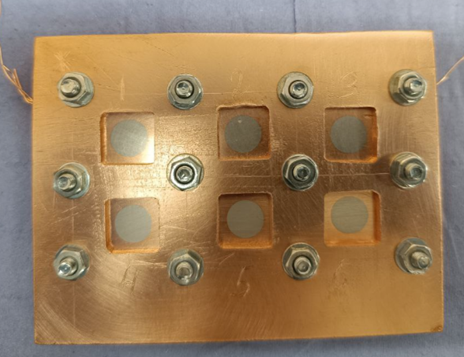
\includegraphics[scale=0.7]{LID_target.png}
    }
    \caption{Вид образцов с пленками вольфрама, расположенных на медном основании. Серые области "--- вольфрам-дейтериевые пленки}\label{fig:ch4/LID_target}
\end{figure}

Пространственный профиль плотности энергии измерялся лазерным анализатором SP620U OPHIR-SPIRICON. Полученный профиль соответствовал распределению Гаусса с усредненным значением полной ширины на уровне $1/e^2$ равным \(\mathrm{FW}=\SI{1}{\milli\metre}\) (удвоенное стандартное отклонение соответственно \SI{0.5}{\milli\meter}). Временные профили лазерного импульса измерялись кремниевым фотодиодом ФДУК-200 в фотогальваническом режиме. Временной профиль имел прямоугольную форму с характерной длительностью нарастания/затухания импульса равной \( \approx \SI{10}{\micro\second} \). Экспериментальный стенд (см. рисунок~\ref{fig:ch4/LID_scheme}) включал в себя оптическую схему на основе двухлинзовой фокусирующей системы Галилея, систему перемещения лазерного луча по поверхности и вакуумный объём ($\approx\SI{70}{\liter}$). Вакуумный объём откачивался турбомолекулярным насосом (Turbovac 90i, Leybold) до базового уровня давления \SI{8e-5}{\pascal}.

\begin{figure}[ht]
    \centerfloat{
        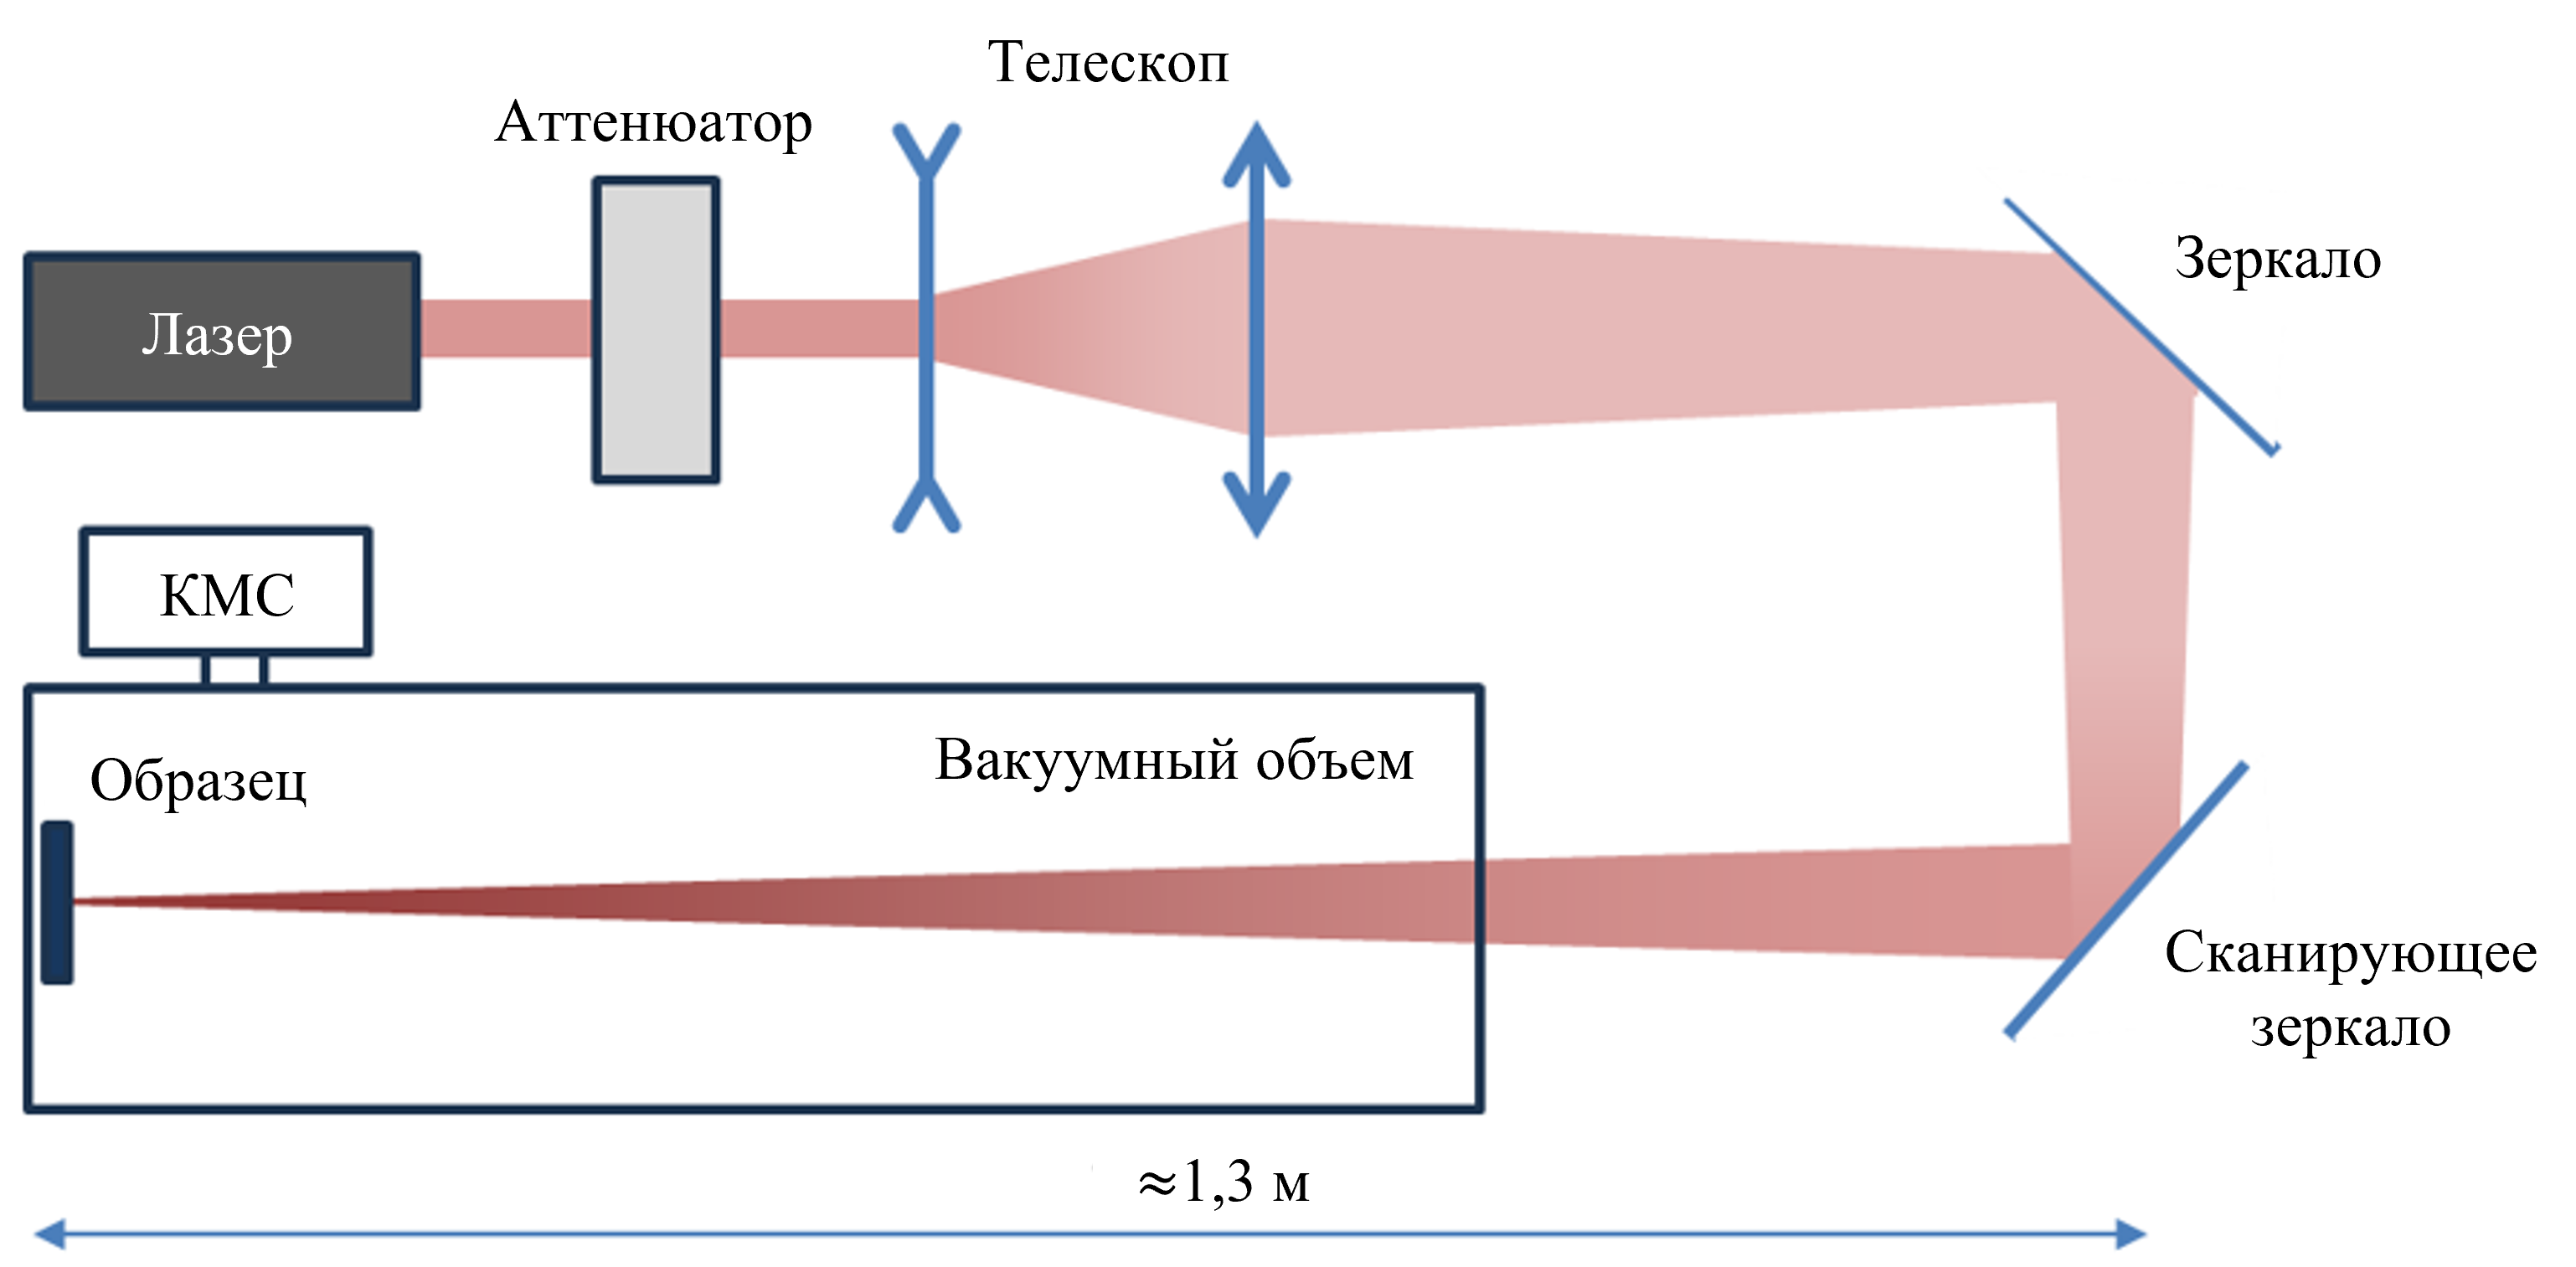
\includegraphics[scale=0.65]{LID_optic_scheme_ru.png}
    }
    \caption{Схема установки для проведения измерений ЛИД~\cite{Medvedev2024}}\label{fig:ch4/LID_scheme}
\end{figure}

Серия измерений при каждой длительности лазерного пучка проводилась на отдельном образце. Участки поверхности образцов облучались серией импульсов с частотой \SI{0.1}{\hertz}. Регистрация сигналов 2; 3 и 4 масс проводилась с помощью КМС (Extorr XT300M). Масс-спектрометр калибровался по постоянному потоку дейтериевой течи с уровнем потока \SI{e-6}{\metre\cubed\pascal\per\second}. В ходе экспериментов изменения в сигналах 3 и 4 масс были ярко выражены, когда сигнал 2-ой массы не отличался от фонового. После серии импульсов энергия лазерного пучка и облучаемая область поверхности менялись. Смещение лазерного пятна происходило на такое расстояние, чтобы избежать влияния предыдущих импульсов на результаты измерений последующих. Для упрощения сравнения результатов численного моделирования с экспериментом из каждой серии импульсов при различных энергиях пучка использовались только первые выстрелы. Откалиброванный сигнал от первого выстрела интегрировался по времени для определения полного числа десорбированных атомов дейтерия. Статистическая погрешность измерений была оценена на уровне 20\%. Температура поверхности образцов в ходе экспериментов не измерялась ввиду ограничений экспериментального стенда.

Получение дополнительной информации о параметрах центров захвата в осажденных пленках осуществлялось методом ТДС. Были исследованы аналогичные образца с соосажденными пленками, толщиной \SI{0.5}{\micro\metre}. Измерения проводились на сверхвысоковакуумном стенде \thesisOrganizationShort \ (кафедра №21)~\cite{Rusinov2009} с постоянной скоростью нагрева \SI{0.5}{\kelvin\per\second}. Сигналы десорбированных молекул регистрировались КМС (HIDEN), работающим с использованием метода пороговой ионизации. Калибровка масс-спектрометра проводилась в соответствии с процедурой, описанной в работе~\cite{Rusinov2009}.

\subsection{Расчетная модель}\label{subsec:ch4/sec1/subsec3}

С целью воспроизведения результатов экспериментальных измерений ЛИД дейтерия из образцов была рассмотрена упрощенная геометрическая модель в цилиндрических координатах с аксиальной симметрией (см. рисунок~\cref{fig:ch4/LID_geom}), состоящая из двух материалов: вольфрамовой пленки (\SI{1}{\micro\meter}) и медной подложки (\SI{6}{\milli\meter}). Радиус расчетной области был выбран равным \SI{2}{\milli\meter}. На таком радиусе интенсивность лазерного импульса существенно затухает (в \( 1/e^{32} \) раз). Характерный масштаб распространения тепла за время лазерного воздействия с миллисекундной длительностью составляет \( L_\mathrm{heat}=\sqrt{\kappa \tau_\mathrm{ms}/C_p \rho} \approx \SI{0.2}{\milli\meter} \), что также не превышает величины радиального размера геометрической модели.

\begin{figure}[ht]
    \centerfloat{
        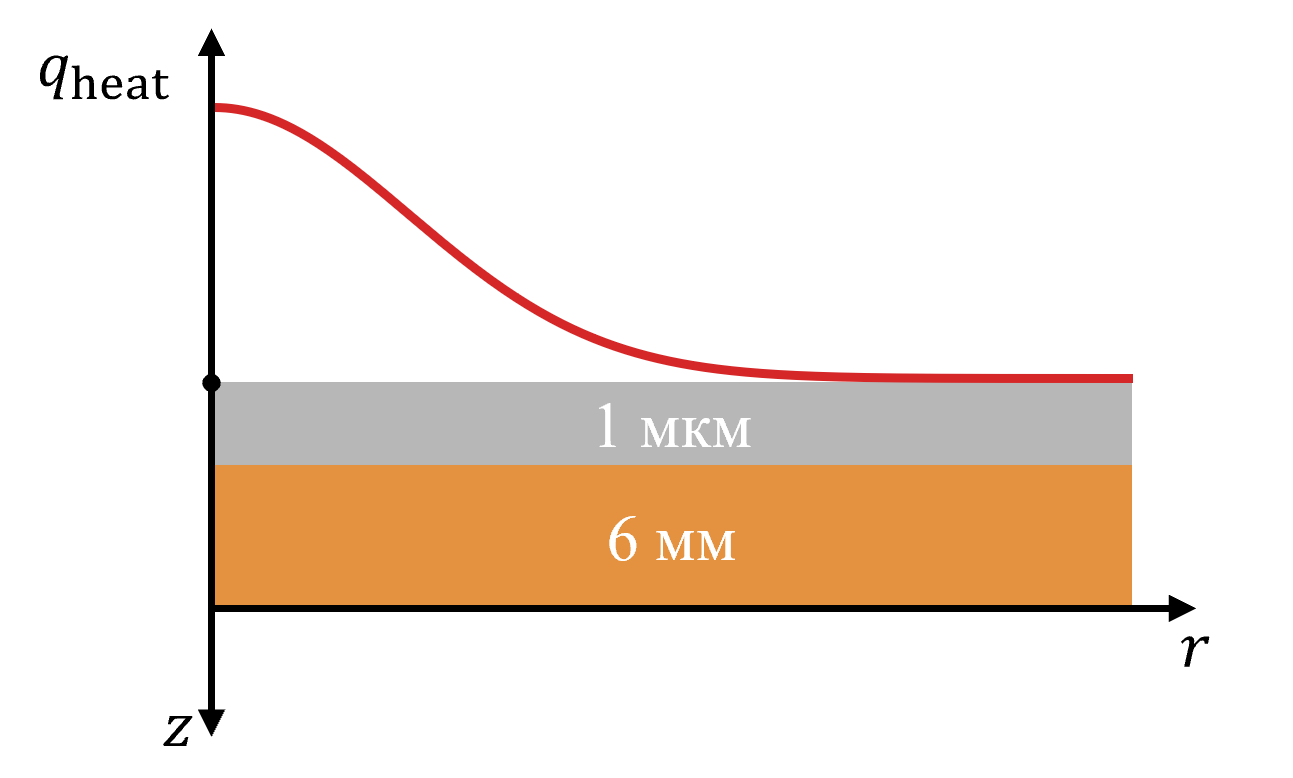
\includegraphics[scale=1]{LID_geom.png}
    }
    \caption{Схематическое представление двумерной геометрической модели, использованной при расчетах ЛИД. Радиус модели \SI{2}{\milli\meter}; \cruleme[customgrey]{0.5cm}{0.5cm}~---~W; \cruleme[customorange]{0.5cm}{0.5cm} "--- Cu}\label{fig:ch4/LID_geom}
\end{figure}

Для проведения численных расчетов было рассмотрено однородное уравнение теплопроводности в приближении идеального теплового контакта между пленкой и подложкой:
\begin{align}
    C_p \rho \frac{\partial T}{\partial t} = \frac{1}{r}\frac{\partial}{\partial r}\left( \kappa r \frac{\partial T}{\partial r} \right) + \frac{\partial }{\partial z}\left( \kappa \frac{\partial T}{\partial z} \right).
\end{align}
Температурная зависимость теплофизических свойств вольфрама и меди определялась уравнениями~\cref{eq:app/W_props,eq:app/Cu_props}. Нагрев за счет лазерного воздействия моделировался в качестве плотности мощности на границе:
\begin{equation}
    -\kappa \left. \frac{\partial T}{\partial z} \right\vert_{z=0} = q(r, t),
\end{equation}
Данное приближение справедливо, когда глубина проникновения лазерного излучения в твердое тело намного меньше характерного пространственного масштаба переноса тепла. Для вольфрама глубина проникновения излучения в ближнем инфракрасном диапазоне составляет величину \( \sim \SI{10}{\nano\meter} \)~\cite{Ordal1988}. Характерный масштаб переноса тепла при микросекундном нагреве можно оценить на уровне \( \sim \SI{0.1}{\milli\meter} \), что подтверждает справедливость приближения. Потерями мощности на излучение пренебрегается по сравнению с лазерным нагревом~\cite{Stepanenko2024}.

Распределение интенсивности лазерного импульса определялось на основе экспериментальных данных:
\begin{equation}
    q(r,t)=\frac{A E_\mathrm{laser}}{2\pi \sigma_{r}^2\tau_\mathrm{imp}} \exp \left( -\frac{r^2}{2 \sigma_r^2} \right) \eta \left( \tau_\mathrm{imp}-t \right),
\end{equation}
где \(A \) "--- коэффициент поглощения лазерного излучения; $E_\mathrm{laser}$ "--- полная энергия лазерного импульса, \si{\joule}; $\sigma_r=\mathrm{FW}/4=\SI{0.25}{\milli\meter}$ "--- стандартное отклонение пространственного распределения; \( \tau_\mathrm{imp} \) "--- длительность лазерного импульса, с; \(\eta(x)\) "--- функция Хевисайда. Передний/задний фронт во временной зависимости интенсивности лазерного импульса не учитывались. На остальных границах температура была фиксирована и равна начальной \(T_0=\SI{300}{\kelvin}\). Коэффициент поглощения лазерного излучения зависит от длины волны, температуры и состояния поверхности. На длине волны \SI{1070}{\nano\meter} он варьируется от \num{0.35} до \num{0.4} в области температур до \( \approx \SI{900}{\kelvin} \)~\cite{Minissale2017}. В ходе экспериментов состояние поверхности и ее температура не контролировались, что не позволяет провести сравнение результатов расчета эволюции температуры материала для уточнения значения параметра. Учитывая метод нанесения пленок, можно предположить, что коэффициент поглощения будет больше, чем в случае чистого вольфрама. В последующей части раздела этот параметр расценивался как свободный.

Задача транспорта дейтерия рассматривалась только для области вольфрама в силу того, что возможное проникновение дейтерия в медь не могло существенно влиять на сигнал измерений в режиме однократного облучения поверхности. Эволюция концентрации подвижных атомов дейтерия определялась из:
\begin{align}
    \frac{\partial \cm}{\partial t} = -\frac{1}{r}\frac{\partial (r J_r )}{\partial r} - \frac{\partial J_z}{\partial z} - \sum\limits_i \frac{\partial \cti}{\partial t},
\end{align}
где компоненты диффузионного потока определяются соответствующими компонентами градиентов концентрации и температуры. Процессы захвата и освобождения из дефектов определялись уравнением~\cref{eq:ch2/trapped_conc}. Полагалось, что все центры захвата распределены равномерно в слое вольфрама, что обычно справедливо для соосажденных пленок~\cite{Krat2020_2}. Начальная концентрация подвижных атомов была равна нулю, когда все дефекты считались полностью заполненными. На облучаемой поверхности задавалась нулевая концентрация подвижных атомов (приближение мгновенной десорбции), когда на остальных границах "--- нулевой поток. Параметры, определяющие транспорт дейтерия и сопутствующие процессы, приведены в таблице~\cref{tab:W_props}. Расчеты проводились на неоднородной сетке, линейный размер элементов которой увеличивался от поверхности вольфрама (\SI{10}{\nano\meter}) до поверхности меди (\SI{0.1}{\milli\meter}). Модельное время составляло \SI{0.1}{\second}, чего было достаточно для окончания десорбции и охлаждения материалов до начальной температуры. Величина временного шага интегрирования во время действия тепловой нагрузки не превышала \num{2.5} и \SI{25}{\micro\second} для микросекундного и миллисекундного случаев.

Определение параметров центров захвата (количество, концентрация, барьер освобождения) проводилось путем анализа ТДС-спектра на основе методики~\cite{Delaporte-Mathurin2021}, описанной ранее в настоящей работе. Моделирование проводилось в одномерном приближении. Температура было однородна по образцу и менялась линейно со временем. Параметры моделирования, граничные и начальные условия для задачи транспорта дейтерия аналогичны тем, что использовались в моделировании ЛИД.

\subsection{Сравнение результатов моделирования и эксперимента}\label{subsec:ch4/sec1/subsec4}

Экспериментальный ТДС-спектр удалось воспроизвести в предположении наличия четырех типов центров захвата:
\begin{enumerate}[beginpenalty=10000]
    \item \( n_\mathrm{t,1}=\SI{2.89}{\text{ат.}\percent} \), \( E_\mathrm{dt,1}=\SI{1.108}{\electronvolt} \);
    \item \( n_\mathrm{t,2}=\SI{1.79}{\text{ат.}\percent} \), \( E_\mathrm{dt,2}=\SI{1.279}{\electronvolt} \);
    \item \( n_\mathrm{t,3}=\SI{1.97}{\text{ат.}\percent} \), \( E_\mathrm{dt,3}=\SI{1.536}{\electronvolt} \);
    \item \( n_\mathrm{t,4}=\SI{0.60}{\text{ат.}\percent} \), \( E_\mathrm{dt,4}=\SI{1.818}{\electronvolt} \).
\end{enumerate}
На рисунке~\cref{fig:ch4/LID_TDS} приведены экспериментальный и модельный ТДС-спектры дейтерия из соосажденных пленок вольфрама. Также явно показан вклад от каждого типа дефекта в поток десорбированных частиц.

\begin{figure}[ht]
    \centerfloat{
        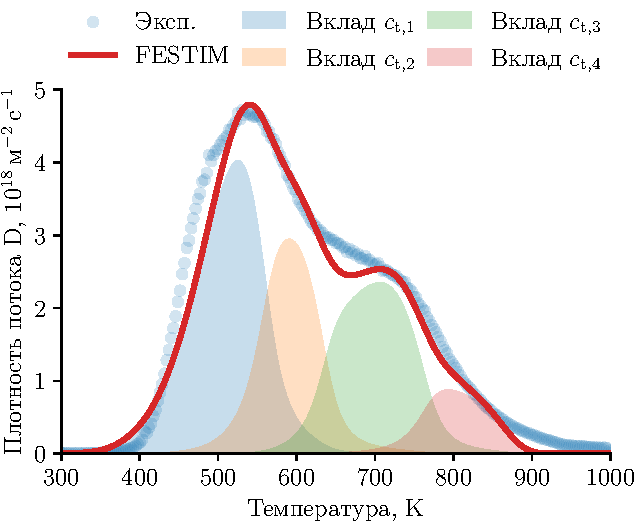
\includegraphics[scale=1]{LID_TDS.pdf}
    }
    \caption{Сравнение ТДС-спектров дейтерия из соосажденных пленок вольфрама, рассчитанного в коде FESTIM и измеренных в эксперименте}\label{fig:ch4/LID_TDS}
\end{figure}

Оцененное содержание дейтерия в пленках составляет более 7 ат.\%. Параметры центров захвата дейтерия согласуются с данными, приведенными в литературе для слоев соосаждения вольфрама~\cite{Krat2018}. Барьер выхода дейтерия \SIrange{1.0}{1.5}{\electronvolt} может соответствовать вакансиям в решетке вольфрама, занятыми одним (\(\approx\SI{1.5}{\electronvolt}\)) или несколькими атомами дейтерия (\(<\SI{1.5}{\electronvolt}\)), когда центр захвата с наибольшим барьером выхода (тип 4) может соответствовать выходу дейтерия из вакансионного кластера~\cite{Ogorodnikova2015}. Полученные параметры дефектов были далее использованы для моделирования ЛИД.

На рисунке~\cref{fig:ch4/LID_2D} показаны распределения поля температуры при достижении максимального значения для двух длительностей лазерного импульса. Максимальная температура в обоих случаях достигается в конце плато импульсов. При фиксированных параметрах образца миллисекундный нагрев приводит к достижению большей температуры материала. Из распределений профилей температуры следует, что во время лазерного воздействия прогревается область с радиусом \( \approx \SI{0.5}{\milli\meter} \). На нижней паре графиков показаны распределения содержания дейтерия после облучения, когда выход дейтерия прекращается. Из сравнения результатов для двух длительностей следует, что при примерно одинаковой пиковой температуре поверхности эффективность ЛИД выше при использовании более длительного импульса. Однако в обоих случаях радиус анализируемой области составляет ≈0,5 мм, что соответствует полуширине пространственного профиля энергии лазерного импульса.

\begin{figure}[ht]
    \centerfloat{
        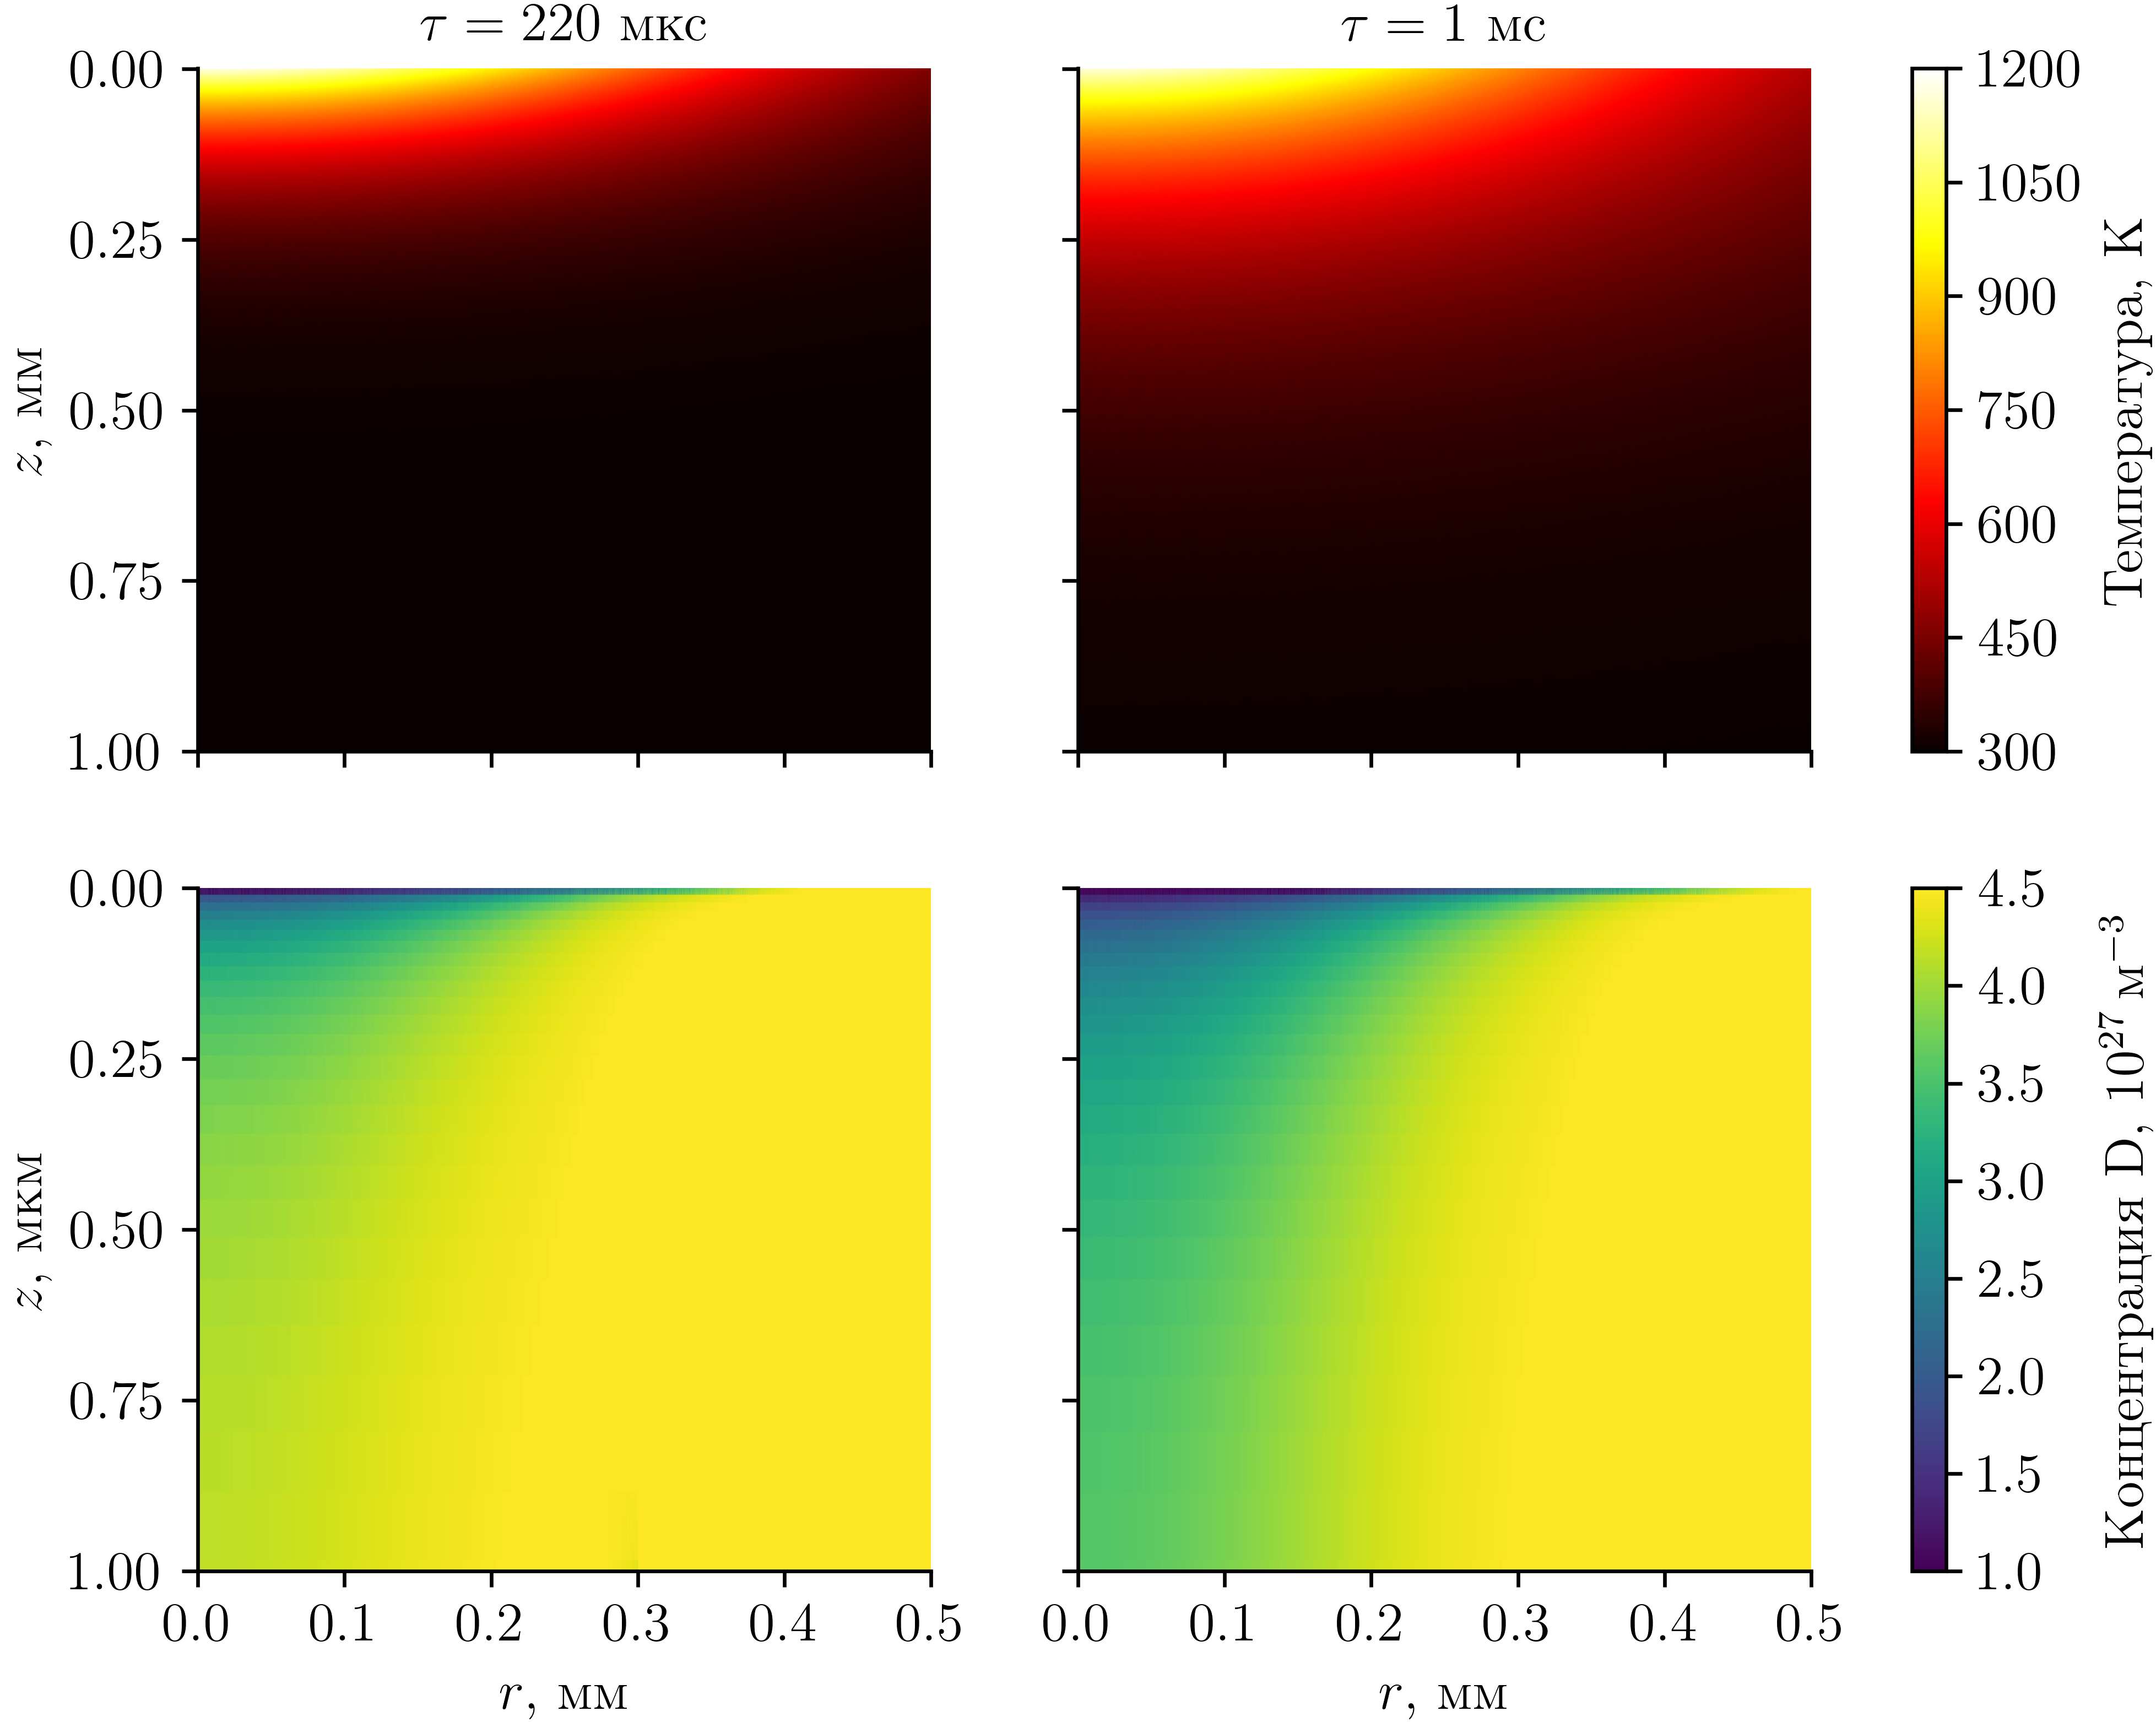
\includegraphics[scale=1]{LID_2D.png}
    }
    \caption{Распределения температуры при достижении максимального значения (вверху) и содержания дейтерия в конце расчета (внизу) для двух длительностей лазерного импульса при \( A = \num{0.55} \)}\label{fig:ch4/LID_2D}
\end{figure}

Была проведена серия расчетов при различных энергиях лазерного импульса для двух длительностей импульсов. Для каждого случая было определено полное число десорбированных атомов дейтерия за импульс. Сравнение результатов моделирования и экспериментальных измерений представлено на рисунке~\cref{fig:ch4/LID_Comparison}. Результаты, полученные путем моделирования, хорошо согласуются с экспериментальными зависимостями при выборе коэффициента поглощения лазерного излучения равным \(A=\num{0.55}\). Для демонстрации влияния коэффициента на рисунке также приведена область изменения результатов при варьировании параметра от \num{0.5} до \num{0.6}. Для обеих длительностей импульсов наблюдается рост числа вышедших частиц с увеличением энергии, вложенной в лазерный импульс. Число десорбированного дейтерия оказывается выше при предельной тепловой нагрузке в случае использования миллисекундного ЛИД, что демонстрирует влияние длительности лазерного нагрева на эффективность анализа.

\begin{figure}[ht]
    \centerfloat{
        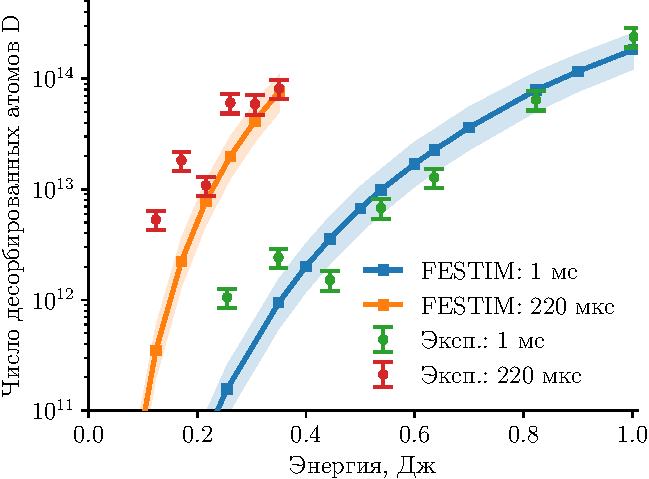
\includegraphics[scale=1]{LID_Comparison.pdf}
    }
    \caption{Сравнение расчетных и экспериментальных зависимостей числа десорбированных частиц от энергии лазерного импульса. Сплошные линии соответствуют коэффициенту поглощения излучения \( A=\num{0.55} \), закрашенные области "--- \( A = \SIrange{0.5}{0.6}{} \)}\label{fig:ch4/LID_Comparison}
\end{figure}

Из сравнения результатов видно, что более хорошее согласие было достигнуто в случае миллисекундного нагрева. Более точное измерение параметров нагрева и/или температуры пленки во время ЛИД (например, температуры ее поверхности) позволит уточнить решение задачи о переносе тепла и минимизировать влияние неизвестных параметров. Учитывая указанную неопределенность, получено хорошее согласие между экспериментальными данными и результатами моделирования на основе стандартной модели транспорта изотопов водорода.

\section{Анализ состава потока десорбированных частиц}\label{sec:ch4/seс2}

Анализ ТДС-экспериментов обычно основывается на предположении о молекулярной рекомбинации на поверхности. Некоторые эмпирические результаты, однако, свидетельствуют о возможности прямой десорбции атомов. Ранее отмечалось, что капиллярные источники атомарного водорода работают на принципе термической диссоциации инжектированных молекул на горячих стенках. Степень атомизации в таких установках может превышать \SI{90}{\percent} при температурах выше \SI{2400}{\kelvin} и плотности потока напускаемого газа \SIrange{e20}{e22}{\per\meter\squared\per\second}~\cite{Tschersich2000,Tschersich2008}.

В условиях ЛИД могут достигаться соизмеримые температуры поверхности, однако плотность потока частиц, десорбированных после мощного лазерного облучения, может на несколько порядков превышать значения, характерные для ТДС, и существенно варьироваться в зависимости от длительности импульса. Так, при использовании коротких (\SI{}{\nano\second}) импульсов плотность потока оценивается на уровне \SI{e27}{\per\meter\squared\per\second}~\cite{Gasparyan2021}, что увеличивает вероятность выхода молекул с поверхности. В то же время, при более длительных импульсах, когда плотность потока оказывается на несколько порядков меньше~\cite{Yu2019}, можно ожидать существенного выхода атомов.

Наличие значительной атомарной фракции в потоке десорбированных частиц может влиять на точность измерений. В ЛИДС количественный анализ числа вышедших атомов основан на измерении фотонного потока, возникающего при их ионизации в пристеночной плазме. Коэффициенты пропорциональности между потоками определяются типом частиц и механизмами их ионизации. В экспериментах на токамаке TEXTOR было зафиксировано увеличение вклада десорбированных атомов (и соответствующее снижение вклада молекул) в регистрируемый фотонный поток при повышении температуры графитового лимитера~\cite{Brezinsek2005}. Было сделано предположении о росте роли десорбции атомов с более горячей поверхности. В качестве основных механизмов рождения фотонов указываются ионизация атомов электронным ударом и диссоциация молекул после ионизации электронным ударом, что в обоих случаях приводит к эмиссии одного фотона и требует учета для корректной интерпретации спектроскопических измерений. Следует подчеркнуть, что пример приведен для графитовой поверхности, процессы десорбции изотопов водорода с которой отличаются от случая металлических поверхностей. Однако процедура спектроскопических измерений остается прежней.

Выход атомов с поверхности может также вносить погрешность в результаты измерений КМС, поскольку вероятность достижения атомами измерительного прибора может быть меньше, чем в случае молекулы, из-за большего коэффициента прилипания к поверхности. Таким образом, информация о величине атомарной фракции в потоке десорбированных частиц во время ЛИД может иметь значение для проведения точной обработки результатов измерений.

\subsection{Постановка задачи}\label{subsec:ch4/seс2/subsec1}
Оценка атомарной фракции в потоке десорбированных частиц проводилась на основе численной модели ЛИД дейтерия из вольфрама в одномерном приближении~\cite{Kulagin2023}. Данное приближение не влияет на основные выводы раздела и может в разумных пределах воспроизводить результаты двумерных расчетов, когда радиус лазерного пятна превышает характерные масштабы переноса тепла и транспорта дейтерия~\cite{Stepanenko2024}. Задача о переносе тепла определялась аналогично прошлому разделу:
\begin{subequations}
    \label{eq:ch4/LID_heat_equation}
    \begin{align}
        C_p \rho \frac{\partial T}{\partial t}                         & = \frac{\partial}{\partial x}\left( \kappa \frac{\partial T}{\partial x} \right), \\
        -\kappa \left. \frac{\partial T}{\partial x} \right\vert_{x=0} & = \frac{E_0}{\tau_\mathrm{imp}} w(t),
    \end{align}
\end{subequations}
где \( E_0 \) "--- плотность поглощенной энергии лазерного импульса, \si{\joule\per\meter\squared}; \( \tau_\mathrm{imp} \) "--- длительность лазерного импульса, с; \(w(t) \) "--- временной профиль импульса. На обратной стороне температура была фиксирована и равна начальной \(T_0=\SI{300}{\kelvin}\). Теплофизические свойства вольфрама задавались на основе выражений~\cref{eq:app/W_props}.

Чтобы исследовать влияние длительности нагрева, рассматривалось три случая, соответствущих экспериментальным работам~\cite{Zlobinski2019,Zlobinski2020,Gasparyan2021}:
\begin{itemize}
    \item наносекундный нагрев с гауссовым временным профилем при положении максимума \( t_0 = \SI{40}{\nano\second} \) и шириной \(\tau_\mathrm{ns}=\SI{25}{\nano\second} \);
    \item микросекундный нагрев с прямоугольным временным профилем, определяемым кусочно-гладкой функцией~\cref{eq:ch3/pulse_form} при \(\tau_\mathrm{le}=\tau_\mathrm{te}=\SI{0.5}{\micro\second}\), \(t_1=\SI{0.5}{\micro\second}\), \( t_2=\SI{2.5}{\micro\second}\), \( \Delta=\num{0} \);
    \item миллисекундный нагрев с трапециевидным временным профилем, определяемым кусочно-гладкой функцией~\cref{eq:ch3/pulse_form} при \(\tau_\mathrm{le}=\tau_\mathrm{te}=\SI{0.05}{\milli\second}\), \(t_1=\SI{0.25}{\milli\second}\), \( t_2=\SI{4.95}{\milli\second}\), \( \Delta=\num{-0.3} \).
\end{itemize}
Временные профили импульсов представлены на рисунке~\cref{fig:ch4/laser_time_profiles}.
\begin{figure}[ht]
    \centerfloat{
        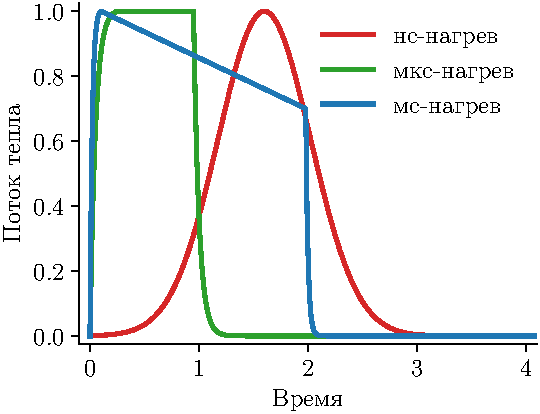
\includegraphics[scale=1]{laser_time_profiles.pdf}
    }
    \caption{Временные зависимости потоков тепла, использованные при моделировании лазерного нагрева различной длительности. Потоки нормированы на максимальное значение.  Длительности импульсов нормированы на \SI{25}{\nano\second}, \SI{10}{\micro\second} и \SI{2.5}{\micro\second} для наносекундного, микросекундного и миллисекундного случаев соответственно. }\label{fig:ch4/laser_time_profiles}
\end{figure}
Предельное значение плотности энергии выбиралось таким образом, чтобы максимальная температура в ходе нагрева не достигала точки плавления. Для нано-, микро-, и миллисекундной длительности она составила величину \SI{10,2}{\kilo\joule\per\meter\squared}; \SI{160.0}{\kilo\joule\per\meter\squared} и \SI{3,8}{\mega\joule\per\meter\squared} соответственно.

В задаче транспорта учитывалось взаимодействие только с одним типом центров захвата (аналогично постановке задачи~\cref{eq:ch3/QSPA_diffusion}), равномерно распределенных в слое толщиной \SI{10}{\micro\meter} с концентрацией \SI{1}{\text{ат.}\percent} и барьером выхода равным \SI{1.5}{\electronvolt}. Данный набор параметров можно отнести к захвату одного атома дейтерия в моновакансиях вольфрама~\cite{Krat2018}. Для анализа состава потока вышедших частиц на левой границе расчетной области рассматривалась модель, учитывающая кинетику процессов на поверхности. В ряде более ранних работ учитывались каналы десорбции молекул с участием как адсорбированных, так и приповерхностных атомов. Обобщение этих механизмов десорбции приведено в работе~\cite{Pisarev1997}. Полагаясь на более раний анализ, в настоящей работе рассматривается три процесса, приводящих к десорбции молекул. Все переходы качественно показаны на рисунке~\cref{fig:ch4/pot_diag_surf}. В явном виде плотность потока частиц в каждом из процессов определяется как:
\begin{subequations}
    \begin{align}
        J_\mathrm{m}^{\mathrm{s}}  & = 2\frac{\csurf^2}{n_\mathrm{s}} \nu_0 \exp \left( -2\frac{E_\mathrm{c}-Q_c(\theta)}{\kBT} \right),                                         \\
        J_\mathrm{m}^{\mathrm{sb}} & = \csurf \frac{\cm}{n_\mathrm{IS}} \nu_\mathrm{D} \exp \left( -\frac{(E_\mathrm{c}-Q_c(\theta))+(E_\mathrm{s}-Q_\mathrm{s})}{\kBT} \right), \\
        J_\mathrm{m}^{\mathrm{b}}  & = 2 \frac{\cm^2}{n_\mathrm{IS}} \lambda_\mathrm{abs} \nu_\mathrm{D} \exp \left( -2\frac{E_\mathrm{s}-Q_\mathrm{s}}{\kBT} \right),
    \end{align}
\end{subequations}
где \( J_\mathrm{m}^{\mathrm{s}} \) "--- поток атомов в составе молекул, формируемый двумя адсорбированными атомами; \( J_\mathrm{m}^{\mathrm{sb}} \) "--- поток атомов в составе молекул, формируемый адсорбированным атомом и растворенным атомом вблизи поверхности; \( J_\mathrm{m}^{\mathrm{b}} \) "--- поток атомов в составе молекул, формируемый двумя растворенными атомами вблизи поверхности; \( \nu_\mathrm{D}=D_0/\lambda_\mathrm{IS}^2 \) "--- характерная частота диффузионных переходов.

Полагается, что в последних двух переходах растворенные атомы рекомбинируют между собой или с адсорбированным атомом и покидают материал, минуя хемосорбированное состояние. Важно подчеркнуть, что данное представление не является точным, так как выражения для констант скоростей процессов, по большей части, дают качественную оценку и построены исходя из размерности величин. Более обоснованное определение возможно, например, на основе DFT-анализа и потребует оценки соответствующих величин при различных конфигурациях атомов как на поверхности, так и в приповерхностном слое, что существенно усложняет задачу.

\begin{figure}[ht]
    \centerfloat{
        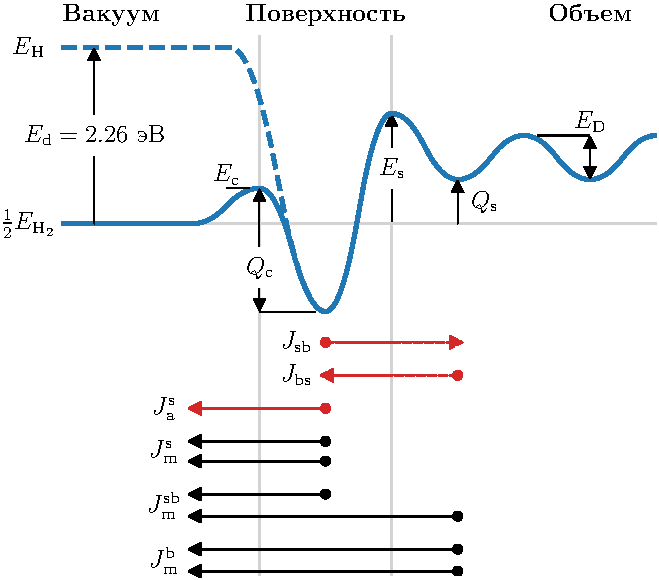
\includegraphics[scale=1]{potential_diagram_surface.pdf}
    }
    \caption{Упрощенная диаграмма потенциальной энергии атома дейтерия вблизи поверхности. Стрелки под диаграммой показывают возможные переходы атомов, учитываемые в моделировании}\label{fig:ch4/pot_diag_surf}
\end{figure}

Для оценки доли атомов в потоке вышедших частиц во время ЛИД была также учтена прямая десорбция атомов с поверхности. Плотность потока атомов определяется аналогично предыдущим величинам:
\begin{equation}
    J_\mathrm{a}^{\mathrm{s}} = \csurf \nu_0 \exp \left( -\frac{E_\mathrm{d}-Q_c(\theta)}{\kBT} \right).
\end{equation}
Во всех выражениях учитывается зависимость теплоты хемосорбции от концентрации адсорбированных атомов аналогично уравнению~\cref{eq:ch2/Edes_coverage} со следующими параметрами~\cite{Hodille2021}: \( Q_\mathrm{0} = \SI{0.071}{\electronvolt} \); \( \Delta Q = \SI{0.647}{\electronvolt} \); \( \theta_0=1.000 \); \( \delta \theta = \num{0.050} \). Эволюция концентрации атомов на поверхности и вблизи (\( x=0 \)) нее определяется следующими дифференциальными выражениями:
\begin{subequations}
    \label{eq:ch4/bcs}
    \begin{align}
        \frac{d \csurf}{dt}                                 & = \Jbs - \Jsb - J_\mathrm{a}^{\mathrm{s}} - J_\mathrm{m}^{\mathrm{s}} - J_\mathrm{m}^{\mathrm{sb}}, \\
        \lambda_\mathrm{IS} \frac{\partial \cm}{\partial t} & = -J_x+ \Jsb - \Jbs - J_\mathrm{m}^{\mathrm{b}} - J_\mathrm{m}^{\mathrm{sb}},
    \end{align}
\end{subequations}
где \( J_x \) "--- компонента диффузионного потока вдоль оси \(x\). В начальный момент времени концентрация дейтерия в объеме и на поверхности была равна нулю. На правой границе также задавалась нулевая концентрация дейтерия.

Значения постоянных, явно не указанные в разделе, обобщены в таблице~\cref{tab:W_props}. Длина расчетной геометрии \( L \) подбиралась таким образом, чтобы температура на правой границе не менялась в ходе моделирования. Она была равна \SI{100}{\micro\meter}; \SI{1}{\milli\meter} и \SI{20}{\milli\meter} для случаев наносекундного, микросекундного и миллисекундного нагрева. Расчеты проводились на неоднородной сетке, размер элементов которой вблизи левой границы не превышал \SI{10}{\nano\meter}. Во время действия тепловой нагрузки временной шаг был не менее чем на два порядка меньше ее характерной длительности.

Искомой величиной в настоящем разделе является атомарная фракция в потоке десорбированного дейтерия, которая определяется как:
\begin{equation}
    f_\mathrm{a} = \dfrac{N_\mathrm{a}}{N_\mathrm{des}}=\dfrac{\int\limits_0^\infty J_\mathrm{a}^\mathrm{s} dt}{\int\limits_0^\infty J_\mathrm{des} dt},
\end{equation}
где $J_\mathrm{des}=J_\mathrm{a}^{\mathrm{s}} + J_\mathrm{m}^{\mathrm{s}} + 2 J_\mathrm{m}^{\mathrm{sb}} + J_\mathrm{a}^{\mathrm{b}}$ "--- плотность полного потока десорбированных атомов.

\subsection{Приближение равновесия процессов вблизи поверхности}\label{subsec:ch4/sec2/subsec2}

Для анализа качественной оценки можно рассмотреть приближение равновесия между концентрациями адсорбированных и растворенных атомов дейтерия~\cite{Kulagin2022a_rus}. В рамках приближения полагается, что равновесие достигается на временном масштабе, который намного меньше характерного времени изменения диффузионного потока у границы и температуры поверхности. Как будет показано в следующем разделе, такие условия могут выполняться в определенных режимах ЛИД. В этих условиях временные производные концентраций равны нулю, а концентрация на некоторой глубине постоянна, что определяет стационарный диффузионный поток. Граничные условия~\cref{eq:ch4/bcs} тогда можно записать в безразмерном виде:
\begin{subequations}
    \begin{align}
        0            & = \omega (1-\theta) k_\mathrm{bs} - \theta (1-\omega) k_\mathrm{sb} - 2\theta^2 k_\mathrm{m}^\mathrm{s} - \theta\omega k_\mathrm{m}^\mathrm{sb} - \theta k_\mathrm{a}^\mathrm{s}, \label{eq:ch4/ss_surface_a} \\
        j_x & = \omega (1-\theta) k_\mathrm{bs} - \theta (1-\omega) k_\mathrm{sb} + 2\omega^2 k_\mathrm{m}^\mathrm{b} +
        \theta\omega k_\mathrm{m}^\mathrm{sb}, \label{eq:ch4/ss_surface_b}
    \end{align}
\end{subequations}
где \( j_x \) "--- безразмерный диффузионный поток; \( k_i \) "--- безразмерная константа скорости перехода. Обезразмеривание было проведено путем деления на величину: \( J_0 = n_\mathrm{s} \nu_0 \). Квазистационарный режим десорбции можно охарактеризовать равновесными степенью покрытия поверхности \( \theta \) и степенью заполнения приповерхностного слоя \( \omega \) с учетом конкретных барьеров перехода, диффузионного потока и температуры.

В общем случае аналитическое решение полученной системы уравнений затруднительно. Однако можно получить некоторые аналитические соотношения. Связь между \( \theta \) и \( \omega \) можно получить из уравнения~\cref{eq:ch4/ss_surface_a}:
\begin{equation}
    \label{eq:ch4/theta_omega_link}
    \omega = \theta \dfrac{2\theta \kms + \kas + k_\mathrm{sb}}{k_\mathrm{bs} - \theta (k_\mathrm{bs} + \kmsb - k_\mathrm{sb})}.
\end{equation}
Соотношение явно указывает на то, что приповерхностная область будет заполняться по мере уменьшения свободных адсорбционных положений. Это позволяет ожидать, что процессы десорбции с участием подповерхностных атомов могут играть роль, когда поверхность насыщается. Если считать, что все процессы, кроме десорбции молекул с поверхности, незначительны, то выражение упрощается до формы, полученной в работе Пика и Сонненберга~\cite{Pick1985}.

Другое очевидное выражение вытекает из разницы между уравнениями~\cref{eq:ch4/ss_surface_b, eq:ch4/ss_surface_a}:
\begin{equation}
    j_x = 2\omega^2 \kmb + 2\theta\omega \kmsb + 2\theta^2 \kms + \theta \kas,
\end{equation}
Здесь правая часть уравнения равна нормализованной плотности полного потока десорбированных атомов \(j_\mathrm{des} \). Члены, пропорциональные \( \omega \), можно опустить, поскольку прямая десорбция атомов ожидается при низкой степени покрытия поверхности и, как следует из уравнения~\cref{eq:ch4/theta_omega_link}, низкой степени заполнения приповерхностной области. В этом случае можно легко получить выражения для степени покрытия поверхности и атомарной фракции:
\begin{subequations}
    \begin{align}
        \theta       & = \frac{\kas}{4 \kms} \left( \sqrt{1+\dfrac{8j_\mathrm{des}\kms}{(\kas)^2}} -1 \right)   \label{eq:ch4/theta_eq}               \\
        f_\mathrm{a} & = \frac{(\kas)^2}{4 j_\mathrm{des} \kms} \left( \sqrt{1+\dfrac{8J_\mathrm{des}\kms}{(\kas)^2}} -1 \right) \label{eq:ch4/at_fr}
    \end{align}
\end{subequations}
Последнее выражение может быть использовано для оценки атомарной фракции в потоке десорбированных частиц, когда поверхность находится ниже насыщения. Оно также отражает увеличение доли атомов с уменьшением общего потока из материала или повышением температуры (\( \kms > (\kas)^2 \)):
\[
    f_\mathrm{a} \propto \sqrt{\dfrac{(\kas)^2}{j_\mathrm{des}\kms}}=\frac{1}{\sqrt{j_\mathrm{des}}} \exp \left( -\frac{E_\mathrm{d}-E_\mathrm{c}}{\kBT} \right).
\]
Примечательно, что приближенное выражение не зависит от теплоты хемосорбции \(Q_\mathrm{c}\). Однако существует экспоненциальная зависимость от барьера хемосорбции \( E_\mathrm{c} \), что позволяет предположить сильное влияние состояния поверхности на соотношение атомов и молекул в потоке десорбированных частиц. Из равенства~\cref{eq:ch4/theta_eq} можно также определить условие достижения насыщения. Полагая левую часть равной единице, приходим к:
\begin{equation}
    j_\mathrm{des}=2\kms+\kas.
\end{equation}

На рисунке~\cref{fig:ch4/atomic_fraction_diagram} приведена диаграмма значений атомарной фракции в зависимости от температуры поверхности и полного потока десорбированных частиц. Диаграмма была построена на основе уравнения~\cref{eq:ch4/at_fr}, которое не учитывает возможное насыщение поверхности. Область применимости ограничена изолинией \(\theta=1\), показанной белой пунктирной линией на рисунке, однако диаграмма остается, в целом корректной, так как в области правее изолинии будет доминировать десорбция молекул.

\begin{figure}[ht]
    \centerfloat{
        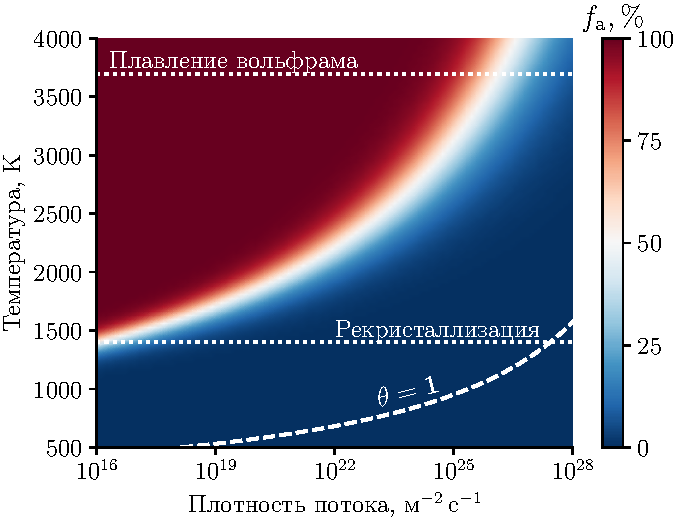
\includegraphics[scale=1]{atomic_fraction_diagram.pdf}
    }
    \caption{Атомарная фракция в приближении равновесия процессов у поверхности при различных значениях температуры и плотности полного потока десорбированных частиц}\label{fig:ch4/atomic_fraction_diagram}
\end{figure}

Согласно диаграмме, доля атомов пренебрежимо мала в условиях, типичных для ТДС-экспериментов: \(J_\mathrm{des} = \SIrange{e16}{e20}{\per\meter\squared\per\second}\) и \( T = \SIrange{400}{1500}{\kelvin} \). В том же диапазоне плотности потока доля атомов возрастает и достигает почти 100\% при температурах более \SI{1500}{\kelvin}. Этот результат коррелирует с типичными условиями в капиллярных атомизаторах водорода, упомянутых ранее. С увеличением плотности общего потока частиц область доминирования атомов смещается в сторону более высоких температур. В промежуточном диапазоне плотностей потока (\SIrange{e20}{e24}{\per\meter\squared\per\second}), которые могут быть достигнуты при миллисекундном лазерном нагреве, ниже температуры рекристаллизации вольфрама выхода атомов не наблюдается. Однако заметное количество атомов может десорбироваться при высоких температурах. В случае более высоких плотностей потока десорбция атомов может происходить только при приближении к температуре плавления вольфрама.

Подводя итоги, можно отметить, десорбция молекул является основным процессом при высоких плотностях потока, тогда как атомная фракция становится значимой только при сравнительно высоких температурах. Однако такие температуры вполне могут быть достигнуты во время ЛИД изотопов водорода из вольфрама. Для количественной оценки необходимо учитывать временные зависимости температуры и потоков частиц: во время лазерного импульса поток частиц может достичь своего пика ещё до максимума температуры поверхности, что повлияет на интегральную величину атомарной фракции.

\subsection{Результаты численного моделирования}\label{subsec:ch4/seс2/subsec3}

Моделирование ЛИД было проведено для всех длительностей лазерного импульса. Характерные временные зависимости плотности потока дейтерия и температуры поверхности  представлены на рисунке~\cref{{fig:ch4/LID_flux}}. Для демонстрации порядка величины плотности потока, достигаемой в ходе ЛИД, результаты приведены только для наносекундной и миллисекундной длительности.

\begin{figure}[ht]
    \centerfloat{
        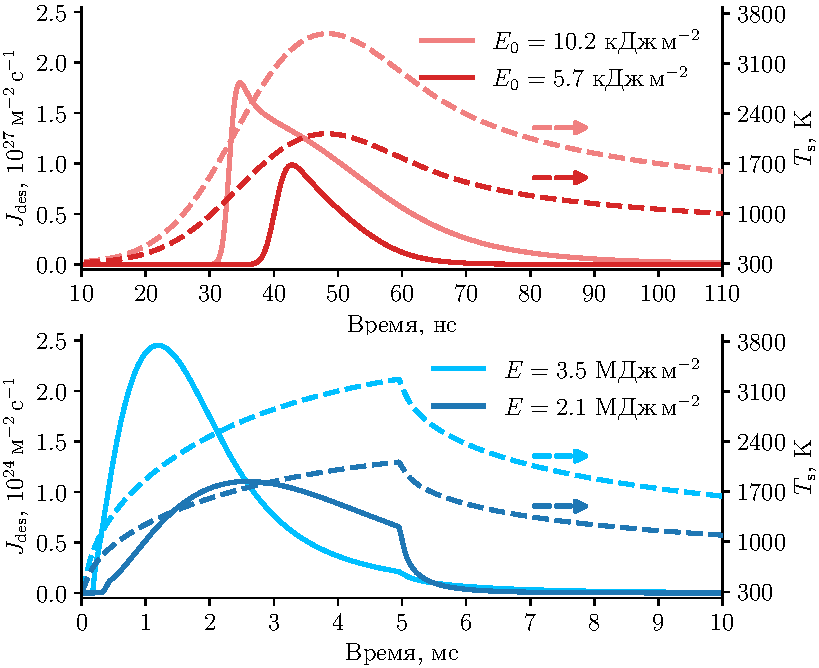
\includegraphics[scale=1]{LID_flux_T_nsms.pdf}
    }
    \caption{Временные зависимости плотности потока десорбированного дейтерия и температуры поверхности вольфрама ($T_\mathrm{s}$) во время нагрева лазерным импульсом с наносекундной и миллисекундной длительностью}\label{fig:ch4/LID_flux}
\end{figure}

На обоих графиках видно, что большая часть атомов дейтерия десорбируется за время лазерного импульса. Наносекундный нагрев приводит к резкому пику плотности потока на уровне \SIrange{e26}{e27}{\per\meter\squared\per\second} ввиду высокой скорости нагрева. Временной профиль плотности потока в случае миллисекундного нагрева имеет характерный пик при наибольшей плотности энергии, когда менее интенсивный нагрев приводит к более плоскому профилю. Величина плотности потока частиц достигает порядка \SIrange{e23}{e24}{\per\meter\squared\per\second}. В обоих сценариях максимум плотности потока атомов достигается до пика температуры. При более высоких плотностях энергии временная задержка между пиками десорбции и температуры увеличивается, что необходимо учитывать для получения количественных оценок.

Выход дейтерия определяется температурой материала и длительностью поддержания этой температуры. В работах~\cite{VanEden2014,Yu2015} было показано, что максимальная температура поверхности может быть использована в качестве характеристики шероховатости поверхности материалов, развивающейся после воздействия импульсных тепловых нагрузок. Аналогичным образом можно поступить для описания интегральных величин в ходе ЛИД. В первом приближении изменение температуры поверхности за счет потока тепла может быть оценено из уравнения теплопроводности с постоянными теплофизическими свойствами материала. Если предположить идеальный тепловой контакт между исследуемым слоем и массивной подложкой (толщина намного превосходит характерный масштаб переноса тепла), то решение задачи~\cref{eq:ch4/LID_heat_equation} совпадет с решением задачи о переносе тепла, определенной на полубесконечной области. Изменение температуры поверхности (\( \Delta T_\mathrm{s} = T(0,t)-T_0\)) определятся из свертки потока тепла с функцией Грина задачи~\cite{Bechtel1975}:
\begin{equation}
    \label{eq:ch4/surface_temp}
    \Delta T_\mathrm{s} = \frac{1}{\sqrt{\pi \kappa C_p \rho}} \int\limits_0^t \frac{q(t')}{\sqrt{t-t'}}dt'.
\end{equation}
Как показано в Приложении А, интеграл может быть выражен через табулированные функции для рассмотренных временных профилей тепловой нагрузки. Уравнение~\cref{eq:ch4/surface_temp} демонстрирует, что изменение температуры пропорционально \( E_0 /\sqrt{\tau_\mathrm{imp}\kappa C_p \rho} \), что позволяет более наглядно сравнивать результаты при различных длительностях облучения.

Общее количество атомов, покинувших материал, определяется путем интегрирования потоков атомов дейтерия. На рисунке~\cref{fig:ch4/LID_desorbed_amount} показанные зависимости интегрального числа десорбированных атомов от максимальной температуры поверхности при различных длительностях тепловых импульсов. Максимальная плотность частиц достигает значения \SI{e19}{\per\meter\squared} за один наносекундный лазерный импульс и увеличивается до уровня \SI{e22}{\per\meter\squared} за миллисекундный. Доля десорбированных атомов составляет лишь незначительную часть начального содержания дейтерия в вольфраме при наносекундном облучении, тогда как почти все захваченные атомы десорбируются при наиболее длительном нагреве до температуры равной \SI{3500}{\kelvin}. Это можно заметить из насыщения соответствующей кривой.

\begin{figure}[ht]
    \centerfloat{
        \hfill
        \subcaptionbox[List-of-Figures entry]{\label{fig:ch4/LID_desorbed_amount}}{%
            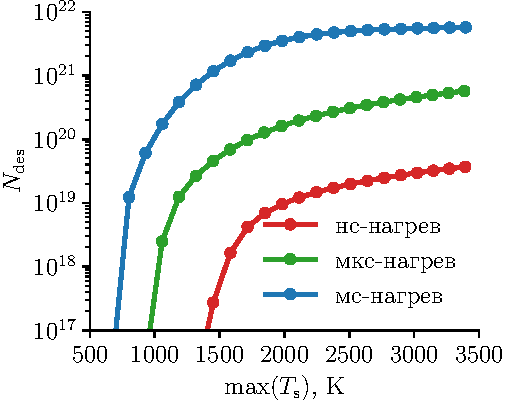
\includegraphics[scale=1]{LID_desorbed_amount}}
        \hfill
        \subcaptionbox{\label{fig:ch4/LID_profiles}}{%
            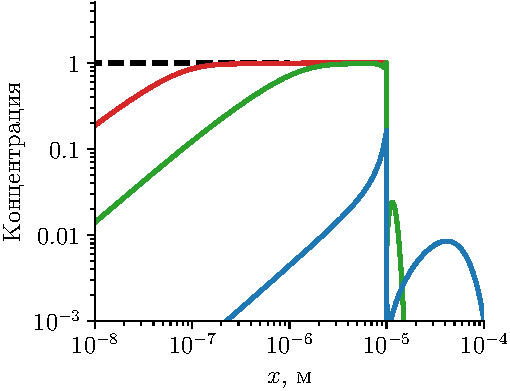
\includegraphics[scale=1]{LID_profiles.pdf}}
    }
    \caption{(а) Зависимость числа десорбированных атомов от максимальной температуры поверхности при нагреве лазерным импульсом с различной длительностью. (б) Пространственное распределение концентрации дейтерия после облучения лазерным импульсом с максимальной плотностью энергии в различных сценариях нагрева. Концентрация дейтерия нормирована на начальное значение}
\end{figure}

Из сравнения распределения содержания дейтерия после облучения (см. рисунок~\cref{fig:ch4/LID_profiles}) можно заключить, что нагрев лазерным импульсом с миллисекундной длительностью более эффективен для анализа толстых поверхностных слоев (\SI{10}{\micro\meter} в рамках модели), а наносекундный ЛИД "--- для изучения тонких поверхностных слоев. Также можно заметить, что в случае нагрева с микро-/миллисекундной длительностью часть атомов мигрирует в объем материала, что вызвано рассмотрением ступенчатого профиля дефектов. В реальных материалах ситуация отличается - они всегда содержат естественные центры захвата, а распределение индуцированных дефектов, образованных нейтронным или ионными облучением, как правило, не имеет резкой границы, что привело бы к заметному снижению скорости распространения атомов за пределы области удержания по сравнению с модельным случаем.

Основной интерес представляет соотношение потоков атомов и молекул, десорбирующихся при лазерном нагреве. Плотность потока десорбированных частиц во время ЛИД лежит в диапазоне от \num{e23} до \SI{e27}{\per\meter\per\second}. Согласно результатам раздела~\cref{sec:ch4/seс2}, десорбция атомов с поверхности ожидается при температурах выше точки рекристаллизации вольфрама. Исходя из этого, основное внимание уделяется сценариям нагрева при наибольшей плотности энергии. На рисунке~\cref{fig:ch4/LID_fluxes} представлены отдельные временные зависимости потоков атомов и молекул при различных длительностях лазерного нагрева. При наносекундном нагреве поток молекул ($J_\mathrm{m}^\mathrm{s}$), состоящий из двух изначально адсорбированных атомов, вносит наибольший вклад в десорбцию даже при температурах, близких к точке плавления. Это довольно ожидаемое наблюдение, поскольку барьер для рекомбинации на поверхности меньше, чем для атомной десорбции. Вдобавок ко всему, степень покрытия поверхности быстро достигает равновесного значения после небольшого снижения после максимума. Поток атомов в этом случае составляет всего несколько процентов от общего потока десорбированных частиц. Аналогичная ситуация наблюдается в случае микросекундного нагрева, однако поток десорбированных атомов на короткий промежуток времени становится соизмерим с молекулярным.

\begin{figure}[ht]
    \centerfloat{
        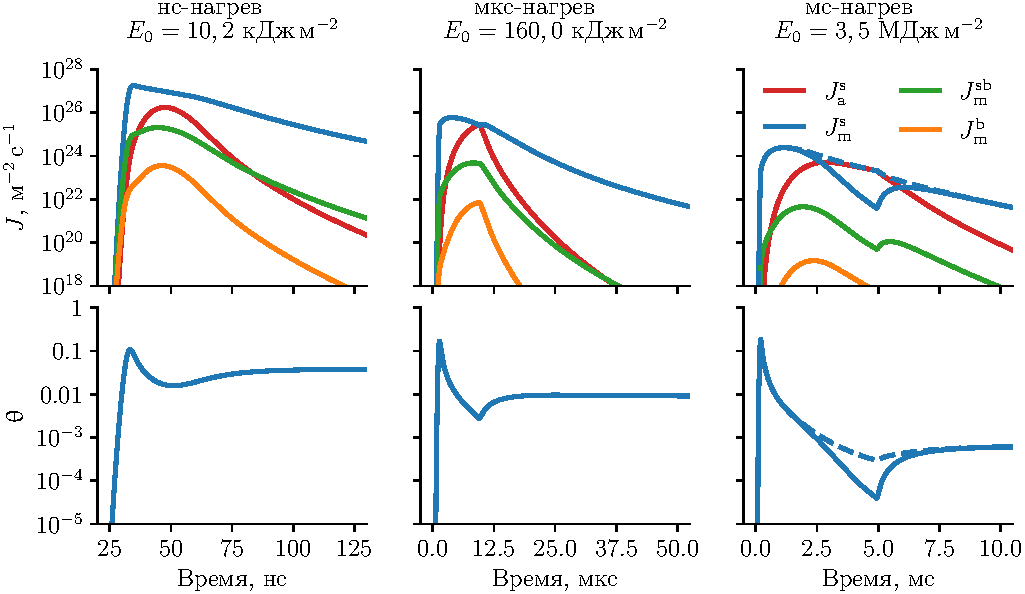
\includegraphics[scale=1]{LID_fluxes.pdf}
    }
    \caption{Временные зависимости потоков атомов (вверху), десорбированных за счет различных механизмов, и степени покрытия поверхности (внизу) при трех длительностях лазерного нагрева. Пунктирные линии показывают изменение соответствующих величин, когда каналы десорбции молекул, включающих растворенные атомы, не учитываются}\label{fig:ch4/LID_fluxes}
\end{figure}

Результаты для миллисекундного нагрева демонстрируют иную динамику процессов десорбции. В начальной фазе, после основного пика, молекулярный поток с поверхности остается преобладающим механизмом десорбции дейтерия вплоть до середины импульса (\( \approx \SI{3}{\milli\second} \)). Однако по мере снижения степени покрытия поверхности интенсивность молекулярного потока быстро уменьшается. В то же время атомный поток, несмотря на умеренное снижение, становится доминирующим благодаря сохранению высокой температуры поверхности. После окончания лазерного воздействия (\SI{5}{\milli\second}) степень покрытия достигает равновесного значения, а температура поверхности падает, что вновь делает молекулярную десорбцию основным механизмом. Для сравнения на рисунке пунктиром показаны временные зависимости потоков десорбированных частиц и степени покрытия в случае, когда учитывается только рекомбинация адсорбированных атомов. В этом сценарии общее количество десорбированного дейтерия сохраняется, но снижение покрытия происходит медленнее.

Из результатов следует, что в условиях ЛИД возможен интервал доминирования прямой десорбции атомов (\SIrange{3}{6}{\milli\second}). В то же время во всех рассмотренных случаях влияние концентрации атомов в приповерхностном слое на расчеты оказалось незначительным. Это указывает на низкое содержание дейтерия в приповерхностной области в рамках данной модели. Для количественной оценки была рассчитана интегральная атомарная фракция для всех длительностей импульса (рисунок~\cref{fig:ch4/LID_atomic_fraction}). Результаты показывают, что доля атомов относительно мала в случае наносекундного нагрева. Их выход инициируется при \SI{2500}{\kelvin}, а её максимальный вклад вблизи температуры плавления не превышает 10\%. С увеличением длительности нагрева температурный порог прямой десорбции смещается в сторону меньших значений. Напротив, в случае микросекундного и миллисекундного нагрева максимальное значение атомарной фракции составляет порядка 10\% от потока десорбированных частиц. Это согласуется с выявленным интервалом доминирования атомной десорбции. При температуре ниже \SI{1500}{\kelvin} десорбция атомов не наблюдается.

\begin{figure}[ht]
    \centerfloat{
        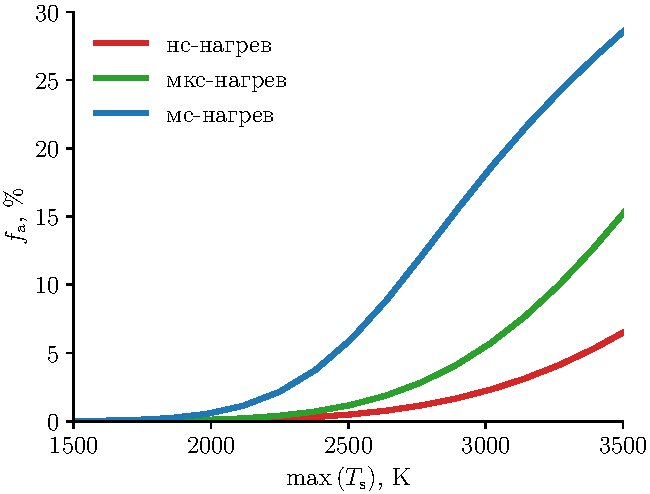
\includegraphics[scale=1]{LID_atomic_fraction.pdf}
    }
    \caption{Зависимости атомарной фракции в потоке десорбированных частиц от максимальной температуры поверхности, достигаемой при лазерном нагреве различной длительности}\label{fig:ch4/LID_atomic_fraction}
\end{figure}

Сравнительный анализ выявил, что значимый вклад атомной десорбции ($\sim\SI{10}{\percent}$) наблюдается исключительно при моделировании высокотемпературного нагрева поверхности ($\max(T_\mathrm{s})>\SI{2500}{\kelvin}$). Следует отметить, что исследование проводилось для фиксированного набора параметров центров захвата. Экстраполяция результатов позволяет предположить, что увеличение концентрации центров захвата или уменьшение энергии связи приведет к снижению атомарной фракции в общем потоке десорбции из-за увеличения потока атомов на поверхность. Особое внимание следует уделить существующей неопределенности в кинетических параметрах модели. Вариации констант скорости поверхностных процессов, в частности рекомбинации и термической десорбции, могут существенно влиять на соотношение между молекулярным и атомарным каналами десорбции. Это ограничение требует дополнительных исследований для уточнения модели.

\section{Анализ влияния параметров материала на выход дейтерия}\label{sec:ch4/seс3}
Напомним, что в установках типа токамак соосаждение изотопов водорода с распыленными атомами материалов первой стенки считается один из основных каналов накопления. Физические свойства соосажденных слоев могут существенно отличаться от характеристик чистых материалов. Более того, разброс параметров, характеризующих содержание изотопов в этих слоях (таких как концентрация ловушек, степень их начального заполнения, энергия связи изотопов с ловушками и др.), влияет на процесс газовыделения, что усложняет получение количественных оценок при интерпретации экспериментальных измерений.

В данном разделе рассматривается влияние параметров материала и центров захвата на эффективность ЛИД дейтерия из вольфрама. Была использована та же модель транспорта дейтерия, что и в предыдущем разделе. Также рассматривался один тип центров захвата, равномерно распределенный в слое толщиной \( L=\SI{10}{\micro\meter}\). Однако был введен дополнительный параметр, определяющий степень начального заполнения центров захвата \(\omega_0 \). Учитывая это, эффективность ЛИД определяется следующим образом:
\begin{equation}
    f_\mathrm{des} = \dfrac{N_\mathrm{des}}{N_0}=\dfrac{\int\limits_0^\infty J_\mathrm{des}dt}{n_\mathrm{t}\omega_0 L}.
\end{equation}
Анализ проводился путем последовательного изменения теплопроводности вольфрама, энергии выхода из центров захвата, концентрации центров захвата и степени их начального заполнения. Все расчеты были проведены для трех длительностей лазерных импульсов. В качестве базовой комбинации параметров были использованы те же параметры, что и раньше: \(E_\mathrm{dt}=\SI{1.5}{\electronvolt} \); \( n_\mathrm{t}=\SI{1}{\text{ат.}\percent} \); \( \omega_0=\SI{100}{\percent} \).

\subsection{Влияние теплопроводности материала}\label{subsec:ch4/seс3/subsec1}

Допустим, исследуемый материал имеет температурную зависимость теплопроводности, аналогичную вольфраму: \( \kappa = a\kappa_\mathrm{W} \), где \(a=\mathrm{const}\). При воздействии лазерного импульса с фиксированными параметрами максимальные изменения температуры поверхности для вольфрамопобного материала и вольфрама соотносятся как: \( \max(\Delta T_\mathrm{s}) = \max(\Delta T_\mathrm{s}^{\mathrm{W}}/\sqrt{a}) \). С одной стороны, это соотношение показывает, что уменьшение теплопроводности будет приводить к увеличению десорбируемой фракции при фиксированном тепловом потоке. С другой стороны, изменение свойств материала влияет на распределение температуры в объеме: \(L_\mathrm{heat}\sim \sqrt{\kappa\tau_\mathrm{imp}/C_p \rho} \). Эквивалентный рост температуры поверхности вольфрамоподобного материала может соответствовать разной глубине, из которой выходит дейтерий. Следовательно, для конкретного значения максимальной температуры следует ожидать некоторый разброс значений эффективности ЛИД.

Описанное выше проиллюстрировано на рисунке~\cref{fig:ch4/LID_kappa_var}. Сплошные линии показывают зависимость количества выделившегося дейтерия от пиковой температуры поверхности чистого вольфрама. Чтобы продемонстрировать влияние тепловых свойств, коэффициент \(a\) варьировался в диапазоне от \num{0.1} до \num{10} при сохранении функциональной зависимости от температуры. Это позволило оценить диапазон изменения эффективности ЛИД (закрашенные области на рисунке) при различных длительностях нагрева. Верхние границы областей соответствуют \( a=\num{10} \), нижние "--- \( a=\num{0.1} \).
\begin{figure}[ht]
    \centerfloat{
        \hfill
        \subcaptionbox[List-of-Figures entry]{\label{fig:ch4/LID_kappavar_a}}{%
            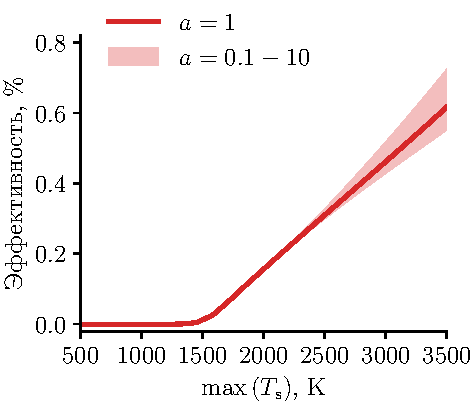
\includegraphics[scale=1]{LID_kappa_var_0.pdf}}
        \hfill
        \subcaptionbox{\label{fig:ch4/LID_kappavar_b}}{%
            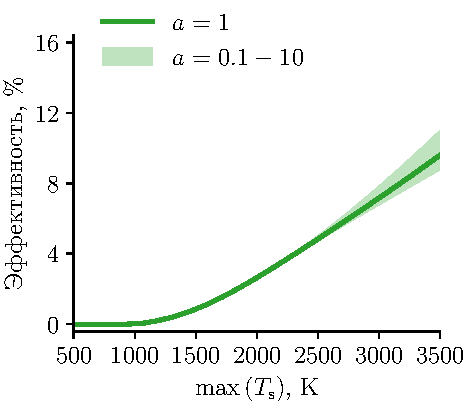
\includegraphics[scale=1]{LID_kappa_var_1.pdf}} \\
        \subcaptionbox{\label{fig:ch4/LID_kappavar_c}}{%
            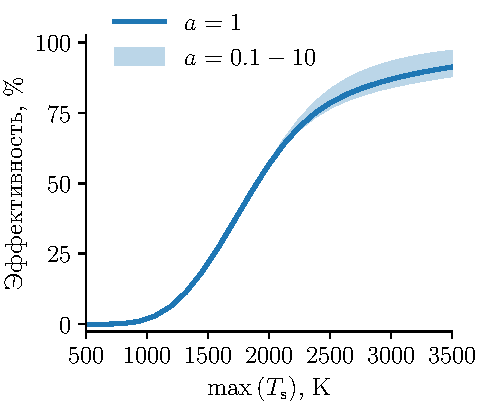
\includegraphics[scale=1]{LID_kappa_var_2.pdf}}
    }
    \caption{Зависимости эффективности ЛИД от максимальной температуры поверхности, достигаемой в наносекундном (а), микросекундном (б) и миллисекундном (в) сценариях нагрева, при различных значениях теплопроводности: \(E_\mathrm{dt}=\SI{1.5}{\electronvolt}\); \(n_\mathrm{t}=\SI{1.0}{\text{ат.}\percent}\); \( \omega_0=\SI{100}{\percent}\)}\label{fig:ch4/LID_kappa_var}
\end{figure}

Рассчитанная эффективность ЛИД для разных значений $a$ характеризуется одинаковой функциональной зависимостью от $\Tsmax$. Большая часть данных совпадает при низких температурах, но в высокотемпературной области наблюдается небольшой разброс. Этот разброс объясняется изменением распределения температуры в объеме. В целом, небольшое изменение свойств материала слабо влияет на результаты, поскольку десорбция дейтерия в основном определяется выходом атомов из наиболее нагретой приповерхностной области (см. профили содержания на рисунке~\cref{fig:ch4/LID_profiles}). Аналогичные рассуждения можно провести для удельной теплоемкости материала. С уменьшением теплоемкости глубина проникновения тепла уменьшается, что должно приводить к снижению эффективности десорбции при фиксированной температуре.

\subsection{Влияние параметров центров захвата}\label{subsec:ch4/seс3/subsec2}

Помимо теплофизических свойств материала, важными факторами, влияющими на высвобождение дейтерия являются параметры центров захвата. В рамках модели, выход из дефектов является единственным источником подвижных атомов дейтерия, поэтому уменьшение энергетического барьера этого процесса ожидаемо повысит интегральный выход. Влияние концентрации ловушек на эффективность ЛИД менее однозначно, поскольку изменение концентрации влияет не только на начальное содержание дейтерия, но и на вероятность его повторного захвата на пути к поверхности. При этом процесс повторного захвата становится более вероятным в случае центров захвата с высокой концентрацией.

Свойства центров захвата дейтерия в материале определяется условиями облучения и/или соосаждения в конкретном эксперименте. В главе~\cref{ch:ch1} было показано, что барьер выхода зависит от типа дефекта и лежит в диапазоне от \(\sim\num{1}\) до \SI{2}{\electronvolt}, когда концентрация центров захвата может достигать нескольких атомных процентов. Соответственно, для анализа влияния параметров дефектов на эффективность ЛИД было проведено две серии расчетов:
\begin{itemize}
    \item с варьированием барьера выхода из дефектов \(E_\mathrm{dt}\) в диапазоне от \(\num{1}\) до \SI{2}{\electronvolt} при их фиксированной концентрации \( n_\mathrm{t}=\SI{1}{\text{ат.}\percent}\);
    \item с варьированием концентрации дефектов \(n_\mathrm{t}\) в диапазоне от \(\num{e-2}\) до \SI{10}{\text{ат.}\percent} при фиксированным барьере выхода \( E_\mathrm{dt}=\SI{1.5}{\electronvolt}\).
\end{itemize}

Моделирование проводилось для всех сценариев нагрева при различных начальных степенях заполнения ловушек $\omega_0$, что позволило охватить широкий диапазон начальных концентраций водорода. На рисунке~\cref{fig:ch4/LID_Edt_n_pop} представлены результаты для случая нагрева поверхности до $\max(T_\mathrm{s}) \approx \SI{3500}{\kelvin}$. Три левых графика показывают зависимость десорбированной фракции от концентрации ловушек $\eta_{tr}$ и их начального заполнения, а три правых отражают влияние барьера выхода из дефектов $E_{dt}$ и начального заполнения. Пунктирные линии соответствуют доле атомов, достигших поверхности, причем расположение графиков отражает возрастание потока на поверхность слева направо.

\begin{figure}[ht]
    \centerfloat{
        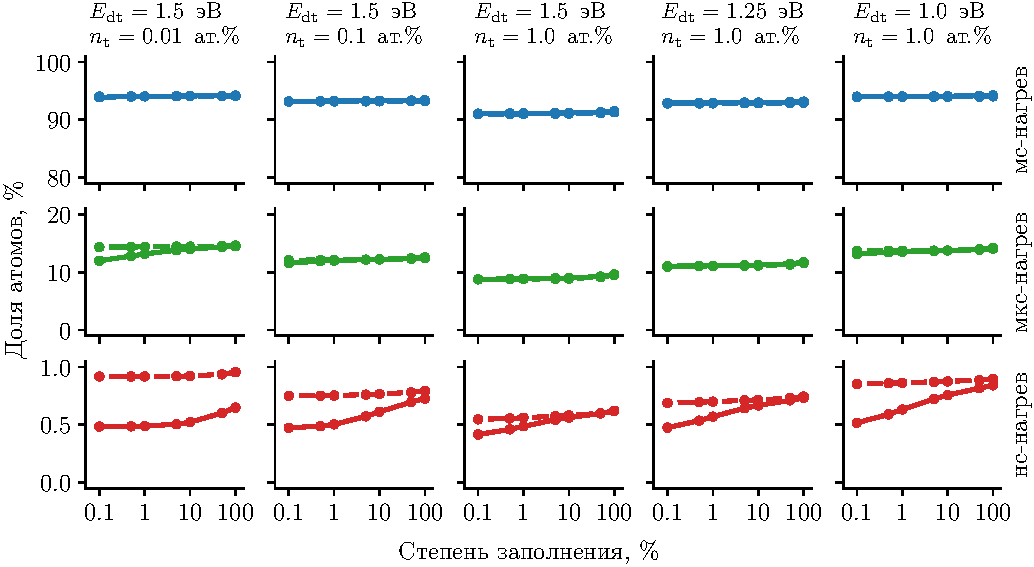
\includegraphics[scale=1]{LID_Edt_n_pop.pdf}
    }
    \caption{Зависимости долей атомов, мигрировавших на поверхность (пунктирные линии) и десорбированных с поверхности (сплошные линии), от начальной степени заполнения центров захвата при различных их параметрах, \(\Tsmax \approx \SI{3500}{\kelvin} \). Плотность энергии составляет \SI{10.2}{\kilo\joule\per\meter\squared}; \SI{160}{\kilo\joule\per\meter\squared} и \SI{3.8}{\mega\joule\per\meter\squared} для наносекундного, микросекундного и миллисекундного нагрева соответственно}\label{fig:ch4/LID_Edt_n_pop}
\end{figure}

Результаты, полученные для различных концентраций ловушек, демонстрируют, что эффективность десорбции снижается с увеличением концентрации центров захвата для всех режимов нагрева. Поэтому можно ожидать меньшей эффективности ЛИД из поверхностных слоев с высоким содержанием дейтерия. Наблюдается систематическое расхождение между долей, десорбированных атомов, и долей, вышедших на поверхность. Разница между этими величинами соответствует доли атомов дейтерия, оставшихся на поверхности. Расхождение присутствует во всех случаях при наносекундном нагреве и в случае центров захвата с низкой концентрацией и неполном начальном заполнении. В первом случае эффект может быть связан с неполной депопуляцией поверхности, как было показано на рисунке~\cref{fig:ch4/LID_fluxes}. Во втором случае эффект вполне ожидаем и связан со снижением вероятности десорбции из-за малой концентрации адсорбированных атомов. Исходя из простой оценки, максимальная степень покрытия поверхности \( \theta \sim L_\mathrm{tr}\omega_0 n_\mathrm{t} / n_\mathrm{s} \ll 1 \). Следовательно, мгновенное значение степени покрытия поверхности в процессе ЛИД также оказывается значительно меньше единицы, что и объясняет наблюдаемое снижение эффективности десорбции.

С другой стороны, эффективность ЛИД возрастает при полном заполнении центров захвата из-за меньшего влияния процесса перезахвата на пути следования к поверхности. При уменьшении барьера выхода из дефектов также наблюдается рост эффективности ЛИД. Однако для $E_{dt}=\SI{1}{\electronvolt}$ при наносекундном нагреве наблюдается неожиданный эффект: несмотря на увеличение потока атомов к поверхности, доля десорбированных атомов резко падает со степенью заполнения. Это объясняется продолжающейся диффузией после импульса, когда атомы легко покидают центры захвата (при низком барьере выхода) и достигают поверхности при температуре, уже недостаточной для десорбции.

В частности, можно отметить, что лишь изменение концентрации центров захвата на несколько порядков способно вызвать сопоставимое изменение эффективности ЛИД, как при увеличении барьера выхода. Очевидно, что влияние концентрации ловушек менее выражено, поскольку вероятность выйти из дефекта экспоненциально зависит от энергетического барьера перехода. В качестве иллюстрации на рисунке~\cref{fig:ch4/LID_n_Edt_var} представлены температурные зависимости эффективности ЛИД при различных параметрах центров захвата. Закрашенные области показывают диапазон изменения значения эффективности при варьировании этих параметров. Обе величины увеличиваются от верхней границы к нижней. Данные расчеты выполнены относительно референсных кривых (сплошные линии), рассчитанных для \(n_\mathrm{t}=\SI{1}{\text{ат.\percent}}\) и \(E_\mathrm{dt}=\SI{1}{\electronvolt}\).

\begin{figure}[ht]
    \centerfloat{
        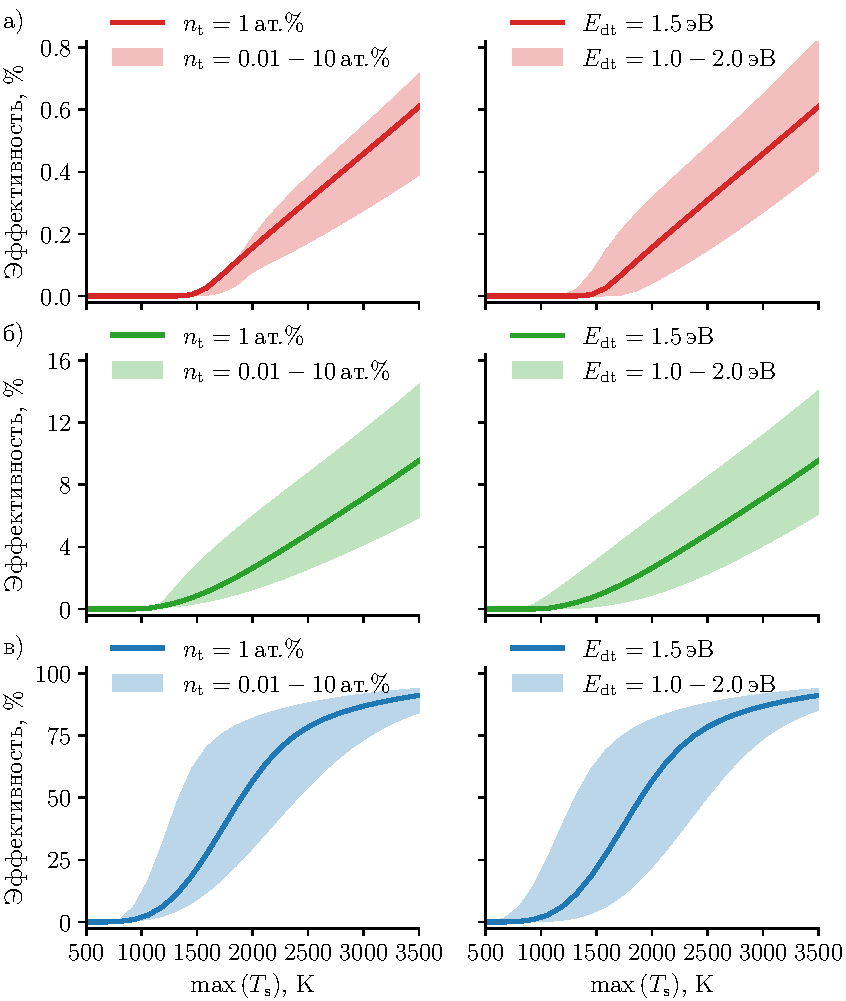
\includegraphics[scale=1]{LID_n_Edt_var.pdf}
    }
    \caption{Зависимости эффективности ЛИД от максимальной температуры поверхности вольфрама, достигаемой в наносекундном (а), микросекундном (б) и миллисекундном (в) сценариях нагрева, при различных параметрах центров захвата: \( \omega_0=\SI{100}{\percent}\)}\label{fig:ch4/LID_n_Edt_var}
\end{figure}

На основании полученных результатов можно выявить несколько качественных закономерностей. Во-первых, десорбция оказывается более эффективной в случае слабых ловушек с низкой концентрацией в широком температурном диапазоне. Следовательно, верхние и нижние границы на графиках иллюстрируют лишь условные пределы возможных значений. Например, эффективность ЛИД в случае дефектов с меньшей концентрацией или более слабыми ловушками может превышать представленные верхние границы. Во-вторых, изменение свойств центров захвата влияет на скорость роста эффективности и, как следствие, на пороговое значение температуры. Таким образом, максимальный разброс значений для всех сценариев нагрева наблюдается при низких температурах и уменьшается для более горячих режимов. Наконец, совпадение эффективностей ЛИД при различных комбинациях (\(n_\mathrm{t}, E_\mathrm{dt}\)) соответствует разному числу десорбированных атомов дейтерия, что указывает на универсальность параметра эффективности.

Отдельного внимания заслуживают данные, представленные в ряду (в) рисунка~\cref{fig:ch4/LID_n_Edt_var}. Они однозначно демонстрируют, что использование более длительных тепловых импульсов повышает эффективность высвобождения. Однако также становится очевидным, что 100\%-ная эффективность десорбции из толстого слоя, вероятно, не может быть достигнута за один импульс нагрева. Как упоминалось ранее, верхний предел обусловлен диффузией дейтерия за пределы области удержания (см. рисунок~\cref{fig:ch4/LID_profiles}), тогда как нижний определяется присутствием центров захвата большим барьером выхода и высокой концентрацией. Эти ограничивающие факторы указывают на необходимость увеличения длительности нагрева или проведения многократного облучения поверхности для достижения полного выхода захваченных атомов.

\subsection{Режимы лазерно-индуцированной десорбции}\label{sec:ch4/seс3/subsec3}

Согласно данным на рисунке~\cref{fig:ch4/LID_Edt_n_pop}, десорбция при лазерном нагреве может быть ограничена процессами на поверхности. Можно выделить два режима, классифицируемых в зависимости от того, процессы в объеме (диффузионные) или на поверхности (десорбционные) определяют выход дейтерия из вольфрама~\cite{Guterl2019}. В первом случае десорбция происходит быстрее, чем диффузия дейтерия из объема. Концентрация дейтерия на поверхности достигает равновесия за характерное время, сопостовимое с изменением диффузионного потока вблизи поверхности. Следовательно, эволюцию поверхностной концентрации дейтерия можно считать квазистационарной. В рамках квазистатического приближения поток десорбированных атомов равен диффузионному: \( J_\mathrm{des}\approx J_{x} \). В противоположном случае поток десорбированных частиц определяется временной эволюцией концентрации атомов на поверхности.

Предполагая, что десорбция происходит только с участием адсорбированных атомов, характерное время процесса (\( \tau_\mathrm{des} \)) можно оценить из следующего выражения:
\begin{equation}
    \label{eq:ch4/des_rate}
    \tau_\mathrm{des}^{-1} \sim \dfrac{\nu_\mathrm{a}^\mathrm{s}}{2} \left( 1 + \sqrt{1+\dfrac{8J_\mathrm{des}\nu_\mathrm{m}^\mathrm{s}}{(\nu_\mathrm{a}^\mathrm{s})^2}} \right),
\end{equation}
где \( \nu_\mathrm{a}^\mathrm{s} \) "--- константа скорости прямой десорбции атомов с поверхности; \( \nu_\mathrm{m}^\mathrm{s} \) "--- константа скорости десорбции атомов в составе молекул с поверхности; \( J_\mathrm{des} \) "--- полный поток десорбированных частиц. Характерное время диффузионного переноса можно оценить на основе эффективного коэффициента диффузии, учитывающего влияние центров захвата:
\begin{subequations}
    \begin{align}
        \tau_\mathrm{D}         & \sim \frac{\delta_\mathrm{eff}^2}{D_\mathrm{eff}}, \\
        D_\mathrm{eff} & = \dfrac{D}{1+\dfrac{n_\mathrm{t}\nu_\mathrm{t}}{\nu_\mathrm{dt}}}. 
    \end{align}
\end{subequations}
Если в приповерхностной области градиент температуры мал, то поток атомов за счет термодиффузии мал, а эффективная длина диффузии оценивается как: \( \delta_\mathrm{eff} \sim \sqrt{\int\limits_0^t D_\mathrm{eff}(T_\mathrm{s})dt'}\). Если десорбция атомов незначительна по сравнению с десорбцией молекул (\(\sqrt{J_\mathrm{des}\nu_\mathrm{m}^{\mathrm{s}}} \gg \nu_\mathrm{a}^\mathrm{s}\)), выражение~\cref{eq:ch4/des_rate} упрощается до вида: \( \tau_\mathrm{des} \sim 1/\sqrt{J_\mathrm{des}\nu_\mathrm{m}^{\mathrm{s}}}\)~\cite{Guterl2019}.

Режимы можно разделить на основе безразмерного параметра \( \xi=\tau_\mathrm{D}/\tau_\mathrm{des} \). Десорбция ограничена процессами в объеме, когда \( \xi \gg 1 \), и определяется процессами на поверхности, когда \( \xi \ll 1 \). Таким образом, выход изотопов водорода во время ЛИД можно считать ограниченными объемными процессами, если преобладающая часть атомов десорбируется при \( \xi \gg 1 \). Параметр \( \xi \) определяется временной эволюцией температуры поверхности, интегральным потоком частиц и параметрами центров захвата. Однако можно заметить, что он не зависит от потока частиц, когда в потоке десорбированных частиц доминирует атомарная фракция: \( \nu_\mathrm{a}^\mathrm{s} \gg \sqrt{J_\mathrm{des}\nu_\mathrm{m}^{\mathrm{s}}} \Rightarrow \xi \approx \nu_\mathrm{a}^\mathrm{s}\tau_\mathrm{D} \). Более того, влияние центров захвата становится незначительным, когда \( \nu_\mathrm{dt} \gg \nu_\mathrm{t} n_\mathrm{t} \Rightarrow D_\mathrm{eff} \approx D \). Наконец, параметр \( \xi \) слабо меняется с эффективной длиной диффузии после достижения пиковой температуры, поскольку эффективный коэффициент диффузии экспоненциально уменьшается в фазе охлаждения, а эффективная длина приближается к постоянному значению.

На рисунке~\cref{fig:ch4/LID_regimes_tmp} представлена характерная иллюстрация режимов ЛИД, где с помощью аналитических выражений (приложение~\cref{app:F}) рассчитаны временные зависимости температуры поверхности (пунктирные линии) и параметра \( \xi \) при максимальной температуре поверхности \(\Tsmax=\SI{3500}{\kelvin} \). Временные зависимости температуры поверхности были получены при постоянных значениях теплофизических параметров, рассчитанных при \( T=\SI{1500}{\kelvin} \). Такой выбор <<эффективных>> параметров позволяет воспроизвести эволюцию температуры поверхности (сплошные линии на графиках) при учете температурной зависимости параметров. На нижних графиках цветные линии отображают эволюцию потока десорбции, полученные путем численного моделирования. Эти зависимости соответствуют данным третьей колонки~\cref{fig:ch4/LID_Edt_n_pop} при \( \omega_0=\SI{100}{\percent} \) (сплошные линии) и \( \omega_0=\SI{0.1}{\percent} \) (пунктирные линии).

\begin{figure}[ht]
    \centerfloat{
        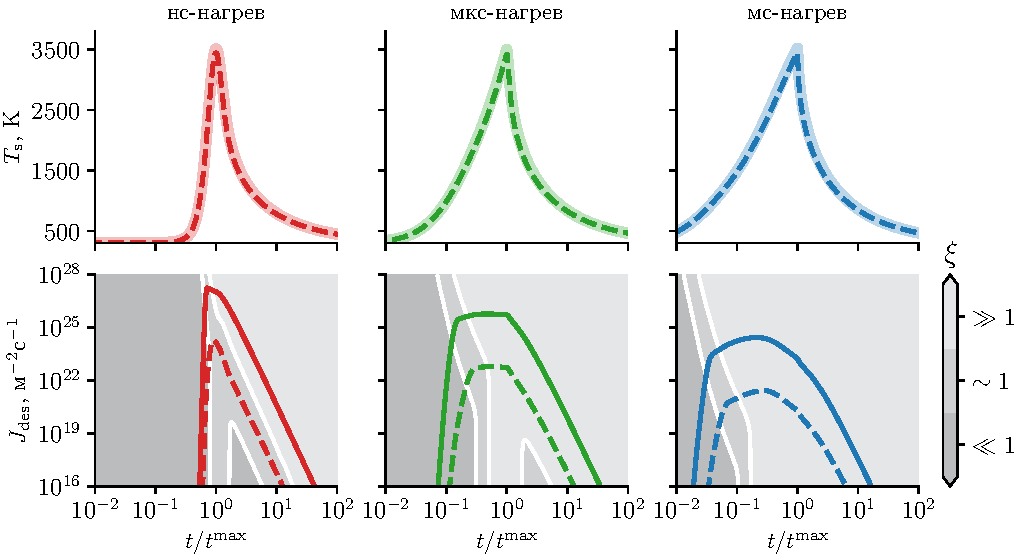
\includegraphics[scale=1.0]{LID_regimes.pdf}
    }
    \caption{Временные зависимости температуры поверхности (верхние графики) и параметра \( \xi \) (нижние графики) при \(\Tsmax=\SI{3500}{\kelvin} \), \( E_\mathrm{dt}=\SI{1.5}{\electronvolt} \) и \(n_\mathrm{t}=\SI{1}{\text{ат.}\percent} \). Пунктирные линии на верхних графиках рассчитаны с помощью аналитических выражений~\cref{eq:dT_ns, eq:dT_usms}, сплошные линии "--- с помощью численного моделирования. Цветные линии на нижних графиках показывают расчетные временные зависимости плотности потока десорбированных частиц при различной начальной степени заполнения центров захвата: сплошные линии соответствуют \( \omega_0=\SI{100}{\percent} \); пунктирные "--- \( \omega_0=\SI{0.1}{\percent} \). Время нормировано на время достижения максимальной температуры \( t^{\mathrm{max}} \)}\label{fig:ch4/LID_regimes_tmp}
\end{figure}

Согласно приведенным диаграммам, ЛИД дейтерия при кратковременном импульсном нагреве ограничивается процессами на поверхности. Объемные процессы могут определять десорбцию лишь при высокой плотности потока , например, при удалении дейтерия из соосажденных слоев с высокой концентрацией захваченных атомов. В то же время более длительный нагрев преимущественно соответствует второму случаю, что обусловлено более долгой диффузией из глубоких слоев области удержания. Данный качественный анализ позволяет лучше объяснить характер зависимостей, представленных на рисунке~\cref{fig:ch4/LID_Edt_n_pop}, где наблюдается расхождение между количеством атомов, мигрировавших на поверхность, и десорбированных с нее. В частности, при микросекундном и миллисекундном нагреве атомы десорбируются преимущественно при \(\xi \gg 1 \),  поэтому интегральное количество десорбированных атомов близко к числу атомов, достигших поверхности (см. центральные панели рисунка~\cref{fig:ch4/LID_Edt_n_pop} для микро-/миллисекундного нагрева). Напротив, в наносекундном режиме нагрева при \( \omega_0=\SI{0.1}{\percent} \) десорбция дейтерия протекает при \(\xi \sim 1 \), вследствие чего доля десорбированных атомов оказывается меньше доли вышедших на поверхность.

Как следствие, длительный нагрев поверхности обеспечивает более высокую эффективность десорбции независимо от поверхностных эффектов. Эти эффекты ограничивают высвобождение атомов при низких потоках десорбированных атомов в условиях изначально свободной поверхности и отсутствия потока адсорбирующихся частиц из вакуума. Если учитывать последний аспект, эффективность десорбции, ограниченной процессами на поверхности, может возрасти благодаря увеличению вероятности молекулярной рекомбинации. С другой стороны, режим ЛИД, когда выход определяют процессы в объеме, позволяет упростить задачу, сведя её к рассмотрению только транспорта дейтерия без учета кинетики процессов на поверхности. Такой подход предоставляет определённые преимущества при интерпретации результатов экспериментальных измерении.

\section{Выводы к главе 4}

В данной части работы проведен комплексный анализ процессов ЛИД дейтерия с поверхности вольфрама методом численного моделирования. Анализ охватил широкий спектр физических процессов и параметров, включая процессы на поверхности, объемные эффекты взаимодействия с дефектами кристаллической решетки, а также влияние характеристик дефектов (энергии связи, концентрации и распределения ловушек). Разработанная модель детально учитывала эти факторы, позволяя анализировать их взаимное влияние на процесс десорбции. Важным этапом исследования стало сравнение результатов моделирования с экспериментальными данными, которое показало их хорошее соответствие, что подтвердило адекватность используемой модели.

Проведённый анализ выявил существенную зависимость атомарной фракции в десорбированном потоке от температуры поверхности и интегральной плотности потока частиц. Установлено, что для импульсов микросекундной длительности и более доля атомарной фракции может достигать величины порядка 10\%, причем этот показатель существенно зависит от параметров процессов на поверхности и содержания дейтерия в материале. Появление значимой фракции атомов в потоке десорбированных частиц может служить дополнительным источником погрешности в ходе экспериментальных измерений.

Последующий анализ показал, что максимальная эффективность ЛИД из толстых поверхностных слоев может быть достигнута при длительном лазерном нагреве материала. Продемонстрированы качественные закономерности изменения эффективности при различных параметрах центров захвата и теплофизических свойств материала. Неопределенность, связанную с параметрами материала, можно минимизировать при проведении измерений температуры поверхности. Однако определяющим фактором является энергетический барьер выхода из центров захвата, малое изменение которого существенно влияет на выход дейтерия из материала, тогда как начальное заполнение ловушек и их концентрация играют меньшую роль. 

Качественный анализ режимов десорбции выявил чёткую зависимость механизма процесса от длительности импульса: при длительности более десяти микросекунд выход дейтерия определяется преимущественно процессами в объеме материала, тогда как для более коротких импульсов лимитирующим фактором становятся процессы на поверхности. Продемонстрировано, что процессы на поверхности могут ограничивать выход дейтерия, что может соответственно снижать эффективность анализа содержания изотопов водорода при использовании коротких длительностей лазерных импульсов.


\clearpage
